% Options for packages loaded elsewhere
\PassOptionsToPackage{unicode}{hyperref}
\PassOptionsToPackage{hyphens}{url}
%
\documentclass[
  12pt,
]{book}
\usepackage{lmodern}
\usepackage{amssymb,amsmath}
\usepackage{ifxetex,ifluatex}
\ifnum 0\ifxetex 1\fi\ifluatex 1\fi=0 % if pdftex
  \usepackage[T1]{fontenc}
  \usepackage[utf8]{inputenc}
  \usepackage{textcomp} % provide euro and other symbols
\else % if luatex or xetex
  \usepackage{unicode-math}
  \defaultfontfeatures{Scale=MatchLowercase}
  \defaultfontfeatures[\rmfamily]{Ligatures=TeX,Scale=1}
\fi
% Use upquote if available, for straight quotes in verbatim environments
\IfFileExists{upquote.sty}{\usepackage{upquote}}{}
\IfFileExists{microtype.sty}{% use microtype if available
  \usepackage[]{microtype}
  \UseMicrotypeSet[protrusion]{basicmath} % disable protrusion for tt fonts
}{}
\makeatletter
\@ifundefined{KOMAClassName}{% if non-KOMA class
  \IfFileExists{parskip.sty}{%
    \usepackage{parskip}
  }{% else
    \setlength{\parindent}{0pt}
    \setlength{\parskip}{6pt plus 2pt minus 1pt}}
}{% if KOMA class
  \KOMAoptions{parskip=half}}
\makeatother
\usepackage{xcolor}
\IfFileExists{xurl.sty}{\usepackage{xurl}}{} % add URL line breaks if available
\IfFileExists{bookmark.sty}{\usepackage{bookmark}}{\usepackage{hyperref}}
\hypersetup{
  pdftitle={BIO8940 Advanced stats and Open Science},
  pdfauthor={Julien Martin},
  hidelinks,
  pdfcreator={LaTeX via pandoc}}
\urlstyle{same} % disable monospaced font for URLs
\usepackage{color}
\usepackage{fancyvrb}
\newcommand{\VerbBar}{|}
\newcommand{\VERB}{\Verb[commandchars=\\\{\}]}
\DefineVerbatimEnvironment{Highlighting}{Verbatim}{commandchars=\\\{\}}
% Add ',fontsize=\small' for more characters per line
\usepackage{framed}
\definecolor{shadecolor}{RGB}{248,248,248}
\newenvironment{Shaded}{\begin{snugshade}}{\end{snugshade}}
\newcommand{\AlertTok}[1]{\textcolor[rgb]{0.94,0.16,0.16}{#1}}
\newcommand{\AnnotationTok}[1]{\textcolor[rgb]{0.56,0.35,0.01}{\textbf{\textit{#1}}}}
\newcommand{\AttributeTok}[1]{\textcolor[rgb]{0.77,0.63,0.00}{#1}}
\newcommand{\BaseNTok}[1]{\textcolor[rgb]{0.00,0.00,0.81}{#1}}
\newcommand{\BuiltInTok}[1]{#1}
\newcommand{\CharTok}[1]{\textcolor[rgb]{0.31,0.60,0.02}{#1}}
\newcommand{\CommentTok}[1]{\textcolor[rgb]{0.56,0.35,0.01}{\textit{#1}}}
\newcommand{\CommentVarTok}[1]{\textcolor[rgb]{0.56,0.35,0.01}{\textbf{\textit{#1}}}}
\newcommand{\ConstantTok}[1]{\textcolor[rgb]{0.00,0.00,0.00}{#1}}
\newcommand{\ControlFlowTok}[1]{\textcolor[rgb]{0.13,0.29,0.53}{\textbf{#1}}}
\newcommand{\DataTypeTok}[1]{\textcolor[rgb]{0.13,0.29,0.53}{#1}}
\newcommand{\DecValTok}[1]{\textcolor[rgb]{0.00,0.00,0.81}{#1}}
\newcommand{\DocumentationTok}[1]{\textcolor[rgb]{0.56,0.35,0.01}{\textbf{\textit{#1}}}}
\newcommand{\ErrorTok}[1]{\textcolor[rgb]{0.64,0.00,0.00}{\textbf{#1}}}
\newcommand{\ExtensionTok}[1]{#1}
\newcommand{\FloatTok}[1]{\textcolor[rgb]{0.00,0.00,0.81}{#1}}
\newcommand{\FunctionTok}[1]{\textcolor[rgb]{0.00,0.00,0.00}{#1}}
\newcommand{\ImportTok}[1]{#1}
\newcommand{\InformationTok}[1]{\textcolor[rgb]{0.56,0.35,0.01}{\textbf{\textit{#1}}}}
\newcommand{\KeywordTok}[1]{\textcolor[rgb]{0.13,0.29,0.53}{\textbf{#1}}}
\newcommand{\NormalTok}[1]{#1}
\newcommand{\OperatorTok}[1]{\textcolor[rgb]{0.81,0.36,0.00}{\textbf{#1}}}
\newcommand{\OtherTok}[1]{\textcolor[rgb]{0.56,0.35,0.01}{#1}}
\newcommand{\PreprocessorTok}[1]{\textcolor[rgb]{0.56,0.35,0.01}{\textit{#1}}}
\newcommand{\RegionMarkerTok}[1]{#1}
\newcommand{\SpecialCharTok}[1]{\textcolor[rgb]{0.00,0.00,0.00}{#1}}
\newcommand{\SpecialStringTok}[1]{\textcolor[rgb]{0.31,0.60,0.02}{#1}}
\newcommand{\StringTok}[1]{\textcolor[rgb]{0.31,0.60,0.02}{#1}}
\newcommand{\VariableTok}[1]{\textcolor[rgb]{0.00,0.00,0.00}{#1}}
\newcommand{\VerbatimStringTok}[1]{\textcolor[rgb]{0.31,0.60,0.02}{#1}}
\newcommand{\WarningTok}[1]{\textcolor[rgb]{0.56,0.35,0.01}{\textbf{\textit{#1}}}}
\usepackage{longtable,booktabs}
% Correct order of tables after \paragraph or \subparagraph
\usepackage{etoolbox}
\makeatletter
\patchcmd\longtable{\par}{\if@noskipsec\mbox{}\fi\par}{}{}
\makeatother
% Allow footnotes in longtable head/foot
\IfFileExists{footnotehyper.sty}{\usepackage{footnotehyper}}{\usepackage{footnote}}
\makesavenoteenv{longtable}
\usepackage{graphicx,grffile}
\makeatletter
\def\maxwidth{\ifdim\Gin@nat@width>\linewidth\linewidth\else\Gin@nat@width\fi}
\def\maxheight{\ifdim\Gin@nat@height>\textheight\textheight\else\Gin@nat@height\fi}
\makeatother
% Scale images if necessary, so that they will not overflow the page
% margins by default, and it is still possible to overwrite the defaults
% using explicit options in \includegraphics[width, height, ...]{}
\setkeys{Gin}{width=\maxwidth,height=\maxheight,keepaspectratio}
% Set default figure placement to htbp
\makeatletter
\def\fps@figure{htbp}
\makeatother
\setlength{\emergencystretch}{3em} % prevent overfull lines
\providecommand{\tightlist}{%
  \setlength{\itemsep}{0pt}\setlength{\parskip}{0pt}}
\setcounter{secnumdepth}{5}
%\usepackage{booktabs}
\usepackage{ctable}
\usepackage{fancyhdr}
\usepackage{float}
\usepackage[margin=2cm]{geometry}

\floatplacement{figure}{H}

%\usepackage[sf,bf]{titlesec}

\hypersetup{colorlinks=true, urlcolor=blue}

\renewcommand{\chaptername}{Chapter}
\renewcommand{\contentsname}{Table of Content}
\renewcommand{\partname}{Part}

\usepackage{framed,color}
\definecolor{incolor}{RGB}{240,240,240}
\definecolor{outcolor}{RGB}{248,248,248}

\renewcommand{\textfraction}{0.05}
\renewcommand{\topfraction}{0.8}
\renewcommand{\bottomfraction}{0.8}
\renewcommand{\floatpagefraction}{0.75}

%\renewenvironment{quote}{\begin{VF}}{\end{VF}}

\ifxetex
 \usepackage{letltxmacro}
 \setlength{\XeTeXLinkMargin}{1pt}
 \LetLtxMacro\SavedIncludeGraphics\includegraphics
 \def\includegraphics#1#{% #1 catches optional stuff (star/opt. arg.)
   \IncludeGraphicsAux{#1}%
 }%
 \newcommand*{\IncludeGraphicsAux}[2]{%
   \XeTeXLinkBox{%
     \SavedIncludeGraphics#1{#2}%
   }%
 }%
\fi

\makeatletter
\newenvironment{kframe}{%
\medskip{}
\setlength{\fboxsep}{.8em}
\def\at@end@of@kframe{}%
\ifinner\ifhmode%
 \def\at@end@of@kframe{\end{minipage}}%
 \begin{minipage}{\columnwidth}%
\fi\fi%
\def\FrameCommand##1{\hskip\@totalleftmargin \hskip-\fboxsep
\colorbox{incolor}{##1}\hskip-\fboxsep
    % There is no \\@totalrightmargin, so:
    \hskip-\linewidth \hskip-\@totalleftmargin \hskip\columnwidth}%
\MakeFramed {\advance\hsize-\width
  \@totalleftmargin\z@ \linewidth\hsize
  \@setminipage}}%
{\par\unskip\endMakeFramed%
\at@end@of@kframe}
\makeatother

\makeatletter
\@ifundefined{Shaded}{
}{\renewenvironment{Shaded}{\begin{kframe}}{\end{kframe}}}
\makeatother

% \let\oldverbatim\verbatim
% \renewenvironment{Shaded}{\vspace{0.2cm}\begin{kframe}}{\end{kframe}}
% \renewenvironment{verbatim}{\begin{shaded}\begin{oldverbatim}}{\end{oldverbatim}\end{shaded}}

\newenvironment{rmdblock}[1]
 {
 \begin{itemize}
 \renewcommand{\labelitemi}{
   \raisebox{-.7\height}[0pt][0pt]{
     {\setkeys{Gin}{width=3em,keepaspectratio}\includegraphics{images/icons/#1}}
   }
 }
 \begin{kframe}
 \setlength{\fboxsep}{1em}
 \item
 }
 {
 \end{kframe}
 \end{itemize}
 }
\newenvironment{rmdnote}
  {\begin{rmdblock}{note}}
  {\end{rmdblock}}
\newenvironment{rmdcaution}
  {\begin{rmdblock}{caution}}
  {\end{rmdblock}}
\newenvironment{rmdimportant}
  {\begin{rmdblock}{important}}
  {\end{rmdblock}}
\newenvironment{rmdtip}
  {\begin{rmdblock}{tip}}
  {\end{rmdblock}}
\newenvironment{rmdwarning}
  {\begin{rmdblock}{warning}}
  {\end{rmdblock}}
\newenvironment{rmdcode}
  {\begin{rmdblock}{code}}
  {\end{rmdblock}}

\usepackage{makeidx}
\makeindex

\urlstyle{tt}

\newcommand{\xelatexemojipath}[1]{images/emoji/#1}

\usepackage{amsthm}
\makeatletter
\def\thm@space@setup{%
  \thm@preskip=8pt plus 2pt minus 4pt
  \thm@postskip=\thm@preskip
}
\makeatother

% \frontmatter
\usepackage{xelatexemoji}
\usepackage[]{natbib}
\bibliographystyle{apalike}

\title{BIO8940 Advanced stats and Open Science}
\usepackage{etoolbox}
\makeatletter
\providecommand{\subtitle}[1]{% add subtitle to \maketitle
  \apptocmd{\@title}{\par {\large #1 \par}}{}{}
}
\makeatother
\subtitle{Work in Progress}
\author{Julien Martin}
\date{09-03-2021}

\begin{document}
\maketitle

%\cleardoublepage\newpage\thispagestyle{empty}\null
%\cleardoublepage\newpage\thispagestyle{empty}\null
%\cleardoublepage\newpage
%\thispagestyle{empty}
%\begin{center}
%
\includegraphics{images/missing.png}
%\end{center}

%\setlength{\abovedisplayskip}{-5pt}
%\setlength{\abovedisplayshortskip}{-5pt}

{
\setcounter{tocdepth}{1}
\tableofcontents
}
\hypertarget{note}{%
\chapter*{Note}\label{note}}
\addcontentsline{toc}{chapter}{Note}

\begin{rmdimportant}
Work in progress. New chapters are going to appears regularly meaning that if you download the pdf it might be incomplete by the time we do the practical in class.
\end{rmdimportant}

\hypertarget{pruxe9face}{%
\chapter*{Préface}\label{pruxe9face}}
\addcontentsline{toc}{chapter}{Préface}

Les exercices de laboratoire que vous retrouverez dans les pages qui suivent sont conçus de manière à vous permettre de développer une expérience pratique en analyse de données à l'aide d'un logiciel (R).
R est un logiciel très puissant, mais comme tous les logiciels, il a des limites.
En particulier il ne peut réfléchir à votre place, vous dire si l'analyse que vous tentez d'effectuer est appropriée ou sensée, ou interpréter biologiquement les résultats.

\hypertarget{quelques-points-importants-uxe0-retenir}{%
\section*{Quelques points importants à retenir}\label{quelques-points-importants-uxe0-retenir}}
\addcontentsline{toc}{section}{Quelques points importants à retenir}

\begin{itemize}
\item
  Avant de commencer une analyse statistique, il faut d'abord vous familiariser son fonctionnement.
  Cela ne veut pas dire que vous devez connaître les outils mathématiques qui la sous-tendent, mais vous devriez au moins comprendre les principes utilisés lors de cette analyse.
  Avant de faire un exercice de laboratoire, lisez donc la section correspondante dans les notes de cours.
  Sans cette lecture préalable, il est très probable que les résultats produits par le logiciel, même si l'analyse a été effectuée correctement, seront indéchiffrables.
\item
  Les laboratoires sont conçus pour compléter les cours théoriques et vice versa.
  À cause des contraintes d'horaires, il se pourrait que le cours et le laboratoire ne soient pas parfaitement synchronisés.
  N'hésitez donc pas à poser des questions sur le labo en classe ou des questions théoriques au laboratoire.
\item
  Travaillez sur les exercices de laboratoire à votre propre rythme.
  Certains exercices prennent beaucoup moins de temps que d'autres et il n'est pas nécessaire de compléter un exercice par séance de laboratoire.
  En fait deux séances de laboratoire sont prévues pour certains des exercices.
  Même si vous n'êtes pas notés sur les exercices de laboratoire, soyez conscient que ces exercices
  sont essentiels.
  Si vous ne les faites pas, il est très peu probable que vous serez capable de compléter les devoirs et le projet de session.
  Prenez donc ces exercices de laboratoire au sérieux !
\item
  Les 2 premier laboratoires sont conçu pour vous permettre d'acquérir ou de réviser le minimum de connaissances requises pour vous permettre de réaliser les exercices de laboratoires avec R.
  Il y a presque toujours de multiples façons de faire les choses avec R et vous ne trouverez ici que des méthodes simples.
  Ceux et celles d'entre vous qui y sont enclins pourront trouver en ligne des instructions plus détaillées et complexes.
  En particulier, je vous conseille :

  \begin{itemize}
  \tightlist
  \item
    R pour les débutants
    \url{http://cran.r-project.org/doc/contrib/Paradis-rdebuts_fr.pdf}
  \item
    An introduction to R
    \url{http://cran.r-project.org/doc/manuals/R-intro.html}
  \item
    Si vous préférez des manuels, le site web de CRAN en garde une liste commentée à :
    \url{http://www.r-project.org/doc/bib/R-books.html}
  \item
    Une liste impressionnante de très bon livre sur R
    \url{https://www.bigbookofr.com/}
  \item
    Finalement, comme aide-mémoire à garder sous la main, je vous recommande R reference card par Tom Short
    \url{http://cran.r-project.org/doc/contrib/Short-refcard.pdf}
  \end{itemize}
\end{itemize}

\hypertarget{quest-ce-que-r-et-pourquoi-lutiliser-dans-ce-cours}{%
\section*{Qu'est-ce que R et pourquoi l'utiliser dans ce cours?}\label{quest-ce-que-r-et-pourquoi-lutiliser-dans-ce-cours}}
\addcontentsline{toc}{section}{Qu'est-ce que R et pourquoi l'utiliser dans ce cours?}

R est un logiciel libre et multi-plateforme formant un système statistique et graphique.
R est également un langage de programmation spécialisé pour les statistiques.

R a deux très grands avantages pour ce cours, et un inconvénient embêtant initialement mais qui vous forcera à acquérir des excellentes habitudes de travail.
Le premier avantage est que vous pouvez tous l'installer sur votre (ou vos) ordinateurs personnel gratuitement.
C'est important parce que c'est à l'usage que vous apprendrez et maîtriserez réellement les biostatistiques et cela implique que vous devez avoir un accès facile et illimité à un logiciel statistique.
Le deuxième avantage est que R peut tout faire en statistiques.
R est conçu pour être extensible et est devenu l'outil de prédilection des statisticiens mondialement.
La question n'est plus : " Est-ce que R peut faire ceci? ``, mais devient'' Comment faire ceci avec R ".
Et la recherche internet est votre ami.
Aucun autre logiciel n'offre ces deux avantages.

L'inconvénient embêtant initialement est que l'on doit opérer R en tapant des instructions (ou en copiant des sections de code) plutôt qu'en utilisant des menus et en cliquant sur différentes options.
Si on ne sait pas quelle commande taper, rien ne se passe.
Ce n'est donc pas facile d'utilisation à priori.
Cependant, il est possible d'apprendre rapidement à faire certaines des opérations de base (ouvrir un fichier de données, faire un graphique pour examiner ces données, effectuer un test statistique simple).
Et une fois que l'on comprend le principe de la chose, on peut assez facilement trouver sur le web des exemples d'analyses ou de graphiques plus complexes et adapter le code à nos propres besoins.
C'est ce que vous ferez dans le premier laboratoire pour vous familiariser avec R.

Pourquoi cet inconvénient est-il d'une certaine façon un avantage? Parce que vous allez sauver du temps en fin de compte.
Garanti.
Croyez-moi, on ne fait jamais une analyse une seule fois.
En cours de route, on découvre des erreurs d'entrée de données, ou que l'on doit faire l'analyse séparément pour des sous-groupes, ou on obtient des données supplémentaires, ou on fait une erreur.
On doit alors recommencer l'analyse.
Avec une interface graphique et des menus, cela implique recommencer à cliquer ici, entre des paramètres dans des boîtes et sélectionner des boutons.
Chaque fois avec possibilité d'erreur.
Avec une série de commandes écrites, il suffit de corriger ce qui doit l'être puis de copier-coller l'ensemble pour répéter instantanément.
Et vous avez la possibilité de parfaitement documenter ce que vous avez fait.
C'est comme cela que les professionnels travaillent et offrent une assurance de qualité de leurs résultats.

\hypertarget{installation-des-logiciels-nuxe9cessaires}{%
\section*{Installation des logiciels nécessaires}\label{installation-des-logiciels-nuxe9cessaires}}
\addcontentsline{toc}{section}{Installation des logiciels nécessaires}

\hypertarget{r}{%
\subsection*{R}\label{r}}
\addcontentsline{toc}{subsection}{R}

Pour installer R sur un nouvel ordinateur, allez au site \url{http://cran.r-project.org/}.
Vous y trouverez des versions compilées (binaries) ou non (sources) pour votre système d'exploitation de prédilection (Windows, MacOS, Linux).

Note : R a déjà été installé sur les ordinateurs du laboratoire (la version pourrait être un peu plus ancienne, mais cela devrait être sans conséquences).

\hypertarget{text-editor-or-ide}{%
\subsection{Text editor or IDE}\label{text-editor-or-ide}}

Tinn-r
Atom sublime, emacs, vim

\hypertarget{rstudio}{%
\subsubsection*{Rstudio}\label{rstudio}}
\addcontentsline{toc}{subsubsection}{Rstudio}

RStudio est un environnement de développement intégré (IDE) créé spécifiquement pour travailler avec R. Sa popularité connaît une progression foudroyante depuis 2014.
Il permet de consulter dans une interface conviviale ses fichiers de script, la ligne de commande R, les rubriques d'aide,
les graphiques, etc.

RStudio est disponible à l'identique pour les plateformes Windows, OS X et Linux.
Pour une utilisation locale sur son poste de travail, on installera la version libre (Open Source) de RStudio Desktop depuis le site
\url{https://www.rstudio.com/products/rstudio/download/}

\hypertarget{visual-studio-code}{%
\subsubsection*{Visual Studio Code}\label{visual-studio-code}}
\addcontentsline{toc}{subsubsection}{Visual Studio Code}

\hypertarget{tinn-r}{%
\subsubsection*{Tinn-r}\label{tinn-r}}
\addcontentsline{toc}{subsubsection}{Tinn-r}

\hypertarget{paquets-pour-r}{%
\subsection*{Paquets pour R}\label{paquets-pour-r}}
\addcontentsline{toc}{subsection}{Paquets pour R}

\begin{itemize}
\tightlist
\item
  Rmarkdown
\item
  tinytex
\end{itemize}

Ces 2 paquets devrait être installé automatiquement avec RStudio, mais pas toujours. Je vous recommande donc de les installer manuellement. Pour ce faire, simplement copier-coller le texte suivant dans le terminal R.

\begin{Shaded}
\begin{Highlighting}[]
\KeywordTok{install.packages}\NormalTok{(}\KeywordTok{c}\NormalTok{(}\StringTok{"rmarkdown"}\NormalTok{, }\StringTok{"tinytex"}\NormalTok{))}
\end{Highlighting}
\end{Shaded}

\hypertarget{pandoc}{%
\subsection*{pandoc}\label{pandoc}}
\addcontentsline{toc}{subsection}{pandoc}

\hypertarget{latex}{%
\subsection*{laTex}\label{latex}}
\addcontentsline{toc}{subsection}{laTex}

\begin{itemize}
\tightlist
\item
  tinytex
  or others
\end{itemize}

\hypertarget{instructions-guxe9nuxe9rales-pour-les-laboratoires}{%
\section*{Instructions générales pour les laboratoires}\label{instructions-guxe9nuxe9rales-pour-les-laboratoires}}
\addcontentsline{toc}{section}{Instructions générales pour les laboratoires}

\begin{itemize}
\tightlist
\item
  Apporter une clé USB ou son équivalent à chaque séance de laboratoire pour sauvegarder votre travail.
\item
  Lire l'exercice de laboratoire AVANT la séance, lire le code R correspondant et préparer vos questions sur le code.
\item
  Durant les pré-labs, écouter les instructions et posez vos questions au moment approprié.
\item
  Faites les exercices du manuel de laboratoire à votre rythme, en équipe, puis je vous recommande de commencer (compléter?) le devoir.
  Profitez de la présence du démonstrateur et du prof\ldots{}
\item
  Pendant vos analyses, copiez-collez des fragments de sorties de R dans un document (par exemple dans votre traitement de texte favori) et annotez abondamment.
\item
  Ne tapez pas directement vos commandes dans R mais plutôt dans un script.
  Vous pourrez ainsi refaire le labo instantanément, récupérer des fragments de code, ou plus facilement identifier les erreurs dans vos analyses.
\item
  Créez votre propre librairie de fragments de codes (snippets).
  Annotez-là abondamment.
  Vous vous en féliciterez plus tard.
\end{itemize}

\hypertarget{notes-sur-le-manuel}{%
\section*{Notes sur le manuel}\label{notes-sur-le-manuel}}
\addcontentsline{toc}{section}{Notes sur le manuel}

Vous trouverez dans le manuel des explications sur la théorie, du code R, des explications sur R et des exercises.

Le manuel essaie aussi de mettre en évidence le texte de différentes manières.

\begin{rmdcode}
Avec des sections à vous de jouer, ui indique un exercise à faire, idéalement sans regarder la solution qui se trouve plus bas.
\end{rmdcode}

\begin{rmdcaution}
des avertissements
\end{rmdcaution}

\begin{rmdwarning}
des avertissements
\end{rmdwarning}

\begin{rmdimportant}
des points importants
\end{rmdimportant}

\begin{rmdnote}
des notes
\end{rmdnote}

\begin{rmdtip}
et des conseils
\end{rmdtip}
\#\#\# Resources \{-\}

Ce document est généré par l'excellente extension \href{https://bookdown.org/}{bookdown} de \href{https://yihui.name/}{Yihui Xie}. Il est basé sur le précédent manuel de laboratoire \emph{BIO4558 manuel de laboratoire} par Antoine Morin. L'introduction à R est largement reprise de l'excellent manuel de \textbf{Julien Barnier} intitulé \href{https://juba.github.io/tidyverse/}{\emph{Introduction à R et au tidyverse}}

\hypertarget{licence}{%
\subsection*{Licence}\label{licence}}
\addcontentsline{toc}{subsection}{Licence}

Ce document est mis à disposition selon les termes de la \href{http://creativecommons.org/licenses/by-nc-sa/4.0/}{Licence Creative Commons Attribution - Pas d'Utilisation Commerciale - Partage dans les Mêmes Conditions 4.0 International}.

\begin{figure}
\centering

\includegraphics{images/icons/license_cc.png}
\caption{Licence Creative Commons}
\end{figure}

\hypertarget{part-open-science}{%
\part{Open Science}\label{part-open-science}}

\hypertarget{introduction-to-open-science}{%
\chapter{Introduction to open Science}\label{introduction-to-open-science}}

\hypertarget{introduction-to-rmarkdown}{%
\chapter{Introduction to Rmarkdown}\label{introduction-to-rmarkdown}}

\hypertarget{practical}{%
\section{Practical}\label{practical}}

We will create a new Rmarkdown document and edit it using basic \texttt{R} and \texttt{Rmarkdown} functions.

\hypertarget{context}{%
\subsection{Context}\label{context}}

We will use the awesome \texttt{palmerpenguins} dataset 🐧 to explore and visualize data.

These data have been collected and shared by \href{https://www.uaf.edu/cfos/people/faculty/detail/kristen-gorman.php}{Dr.~Kristen Gorman} and \href{https://pal.lternet.edu/}{Palmer Station, Antarctica LTER}.

The package was built by Drs Allison Horst and Alison Hill, check out the \href{https://allisonhorst.github.io/palmerpenguins/}{official website}.

The package \texttt{palmerpenguins} has two datasets:

\begin{itemize}
\tightlist
\item
  \texttt{penguins\_raw} has the raw data of penguins observations (see \texttt{?penguins\_raw} for more info)
\item
  \texttt{penguins} is a simplified version of the raw data (see \texttt{?penguins} for more info)
\end{itemize}

For this exercise, we're gonna use the \texttt{penguins} dataset.

\begin{Shaded}
\begin{Highlighting}[]
\KeywordTok{library}\NormalTok{(palmerpenguins)}
\KeywordTok{head}\NormalTok{(penguins)}
\end{Highlighting}
\end{Shaded}

\begin{verbatim}
## # A tibble: 6 x 8
##   species island bill_length_mm bill_depth_mm flipper_length_~ body_mass_g sex  
##   <fct>   <fct>           <dbl>         <dbl>            <int>       <int> <fct>
## 1 Adelie  Torge~           39.1          18.7              181        3750 male 
## 2 Adelie  Torge~           39.5          17.4              186        3800 fema~
## 3 Adelie  Torge~           40.3          18                195        3250 fema~
## 4 Adelie  Torge~           NA            NA                 NA          NA <NA> 
## 5 Adelie  Torge~           36.7          19.3              193        3450 fema~
## 6 Adelie  Torge~           39.3          20.6              190        3650 male 
## # ... with 1 more variable: year <int>
\end{verbatim}

\hypertarget{questions}{%
\subsection{Questions}\label{questions}}

\textbf{1)} Install the package \texttt{palmerpenguins}.

\begin{Shaded}
\begin{Highlighting}[]
\KeywordTok{install.packages}\NormalTok{(}\StringTok{"palmerpenguins"}\NormalTok{)}
\end{Highlighting}
\end{Shaded}

\textbf{2)}

\begin{itemize}
\tightlist
\item
  Create a new R Markdown document, name it and save it.
\item
  Delete everything after line 12.
\item
  Add a new section title, simple text and text in bold font.
\item
  Compile (``Knit'').
\end{itemize}

\textbf{3)}

\begin{itemize}
\tightlist
\item
  Add a chunk in which you load the \texttt{palmerpenguins}. The corresponding line of code should be hidden in the output.
\item
  Load also the \texttt{tidyverse} suite of packages. Modify the defaults to suppress all messages.
\end{itemize}

\begin{Shaded}
\begin{Highlighting}[]
\BaseNTok{```\{r, echo = FALSE, message = FALSE\}}
\BaseNTok{library(palmerpenguins)}
\BaseNTok{library(tidyverse)}
\BaseNTok{```}
\end{Highlighting}
\end{Shaded}

\textbf{4)} Add another chunk in which you build a table with the 10 first rows of the dataset.

\begin{Shaded}
\begin{Highlighting}[]
\BaseNTok{```\{r\}}
\BaseNTok{penguins %>%}
\BaseNTok{  slice(1:10) %>%}
\BaseNTok{  knitr::kable()}
\BaseNTok{```}
\end{Highlighting}
\end{Shaded}

\textbf{5)} In a new section, display how many individuals, penguins species and islands we have in the dataset. This info should appear directly in the text, you need to use inline code 😄. Calculate the mean of the (numeric) traits measured on the penguins.

\begin{Shaded}
\begin{Highlighting}[]
\FunctionTok{## Numerical exploration}

\NormalTok{There are }\BaseNTok{`r nrow(penguins)`}\NormalTok{ penguins in the dataset,}
\NormalTok{and }\BaseNTok{`r length(unique(penguins$species))`}\NormalTok{ different species.}
\NormalTok{The data were collected in }\BaseNTok{`r length(unique(penguins$island))`}
\NormalTok{islands of the Palmer archipelago in Antarctica.}

\NormalTok{The mean of all traits that were measured on the penguins are:}

\BaseNTok{```\{r echo = FALSE\}}
\BaseNTok{penguins %>%}
\BaseNTok{  group_by(species) %>%}
\BaseNTok{  summarize(across(where(is.numeric), mean, na.rm = TRUE))}
\BaseNTok{```}
\end{Highlighting}
\end{Shaded}

\textbf{6)} In another section, entitled `Graphical exploration', build a figure with 3 superimposed histograms, each one corresponding to the body mass of a species.

\begin{Shaded}
\begin{Highlighting}[]
\FunctionTok{## Graphical exploration}

\NormalTok{A histogram of body mass per species:}

\BaseNTok{```\{r, fig.cap = "Distribution of body mass by species of penguins"\}}
\BaseNTok{  ggplot(data = penguins) +}
\BaseNTok{  aes(x = body_mass_g) +}
\BaseNTok{  geom_histogram(aes(fill = species),}
\BaseNTok{                 alpha = 0.5,}
\BaseNTok{                 position = "identity") +}
\BaseNTok{  scale_fill_manual(values = c("darkorange","purple","cyan4")) +}
\BaseNTok{  theme_minimal() +}
\BaseNTok{  labs(x = "Body mass (g)",}
\BaseNTok{       y = "Frequency",}
\BaseNTok{       title = "Penguin body mass")}
\BaseNTok{```}
\end{Highlighting}
\end{Shaded}

\textbf{7)} In another section, entitled \emph{Linear regression}, fit a model of bill length as a function of body size (flipper length), body mass and sex. Obtain the output and graphically evaluate the assumptions of the model. As reminder here is how you fit a linear regression.

\begin{Shaded}
\begin{Highlighting}[]
\BaseNTok{```\{r\}}
\BaseNTok{model <- lm(Y ~  X1 + X2, data = data)}
\BaseNTok{summary(model)}
\BaseNTok{plot(model)}
\BaseNTok{```}
\end{Highlighting}
\end{Shaded}

\begin{Shaded}
\begin{Highlighting}[]
\FunctionTok{## Linear regression}

\NormalTok{And here is a nice model with graphical output}

\BaseNTok{```\{r, fig.cap = "Checking assumptions of the model"\}}
\BaseNTok{m1 <- lm(bill_length_mm ~  flipper_length_mm + body_mass_g + sex, data = penguins)}
\BaseNTok{summary(m1)}
\BaseNTok{par(mfrow= c(2,2))}
\BaseNTok{plot(m1)}
\BaseNTok{```}
\end{Highlighting}
\end{Shaded}

\textbf{8)} Add references manually or using \texttt{citr} in \texttt{RStudio}.

\begin{enumerate}
\def\labelenumi{\arabic{enumi}.}
\tightlist
\item
  Pick a recent publication from the researcher who shared the data, Dr Kristen Gorman. Import this publication in your favorite references manager (we use Zotero, no hard feeling), and create a bibtex reference that you will add to to the file \texttt{mabiblio.bib}.
\item
  Add \texttt{bibliography:\ mabiblio.bib} at the beginning of your R Markdown document (YAML).
\item
  Cite the reference iin the text using either typing the reference manually or using \texttt{citr}. To use \texttt{citr}, instal it first; if everything goes well, you should see it in the pulldown menu \texttt{Addins} 💪. Then simply use \texttt{Insert\ citations} in the pull-down menu \texttt{Addins}.
\item
  Compile.
\end{enumerate}

\textbf{9)} Change the default citation format (Chicago style) into the The American Naturalist format. It can be found here \url{https://www.zotero.org/styles}. To do soo, add \texttt{csl:\ the-american-naturalist.csl} in the YAML.

\textbf{10)} Build your report in html, pdf and docx format. 🎉

\hypertarget{example-of-output}{%
\subsection*{Example of output}\label{example-of-output}}
\addcontentsline{toc}{subsection}{Example of output}

You can see an example of the \href{data/examples/rmarkdown_practical.Rmd}{Rmarkdown source file} and \href{data/examples/rmarkdown_practical.pdf}{pdf output}

\begin{figure}

{\centering 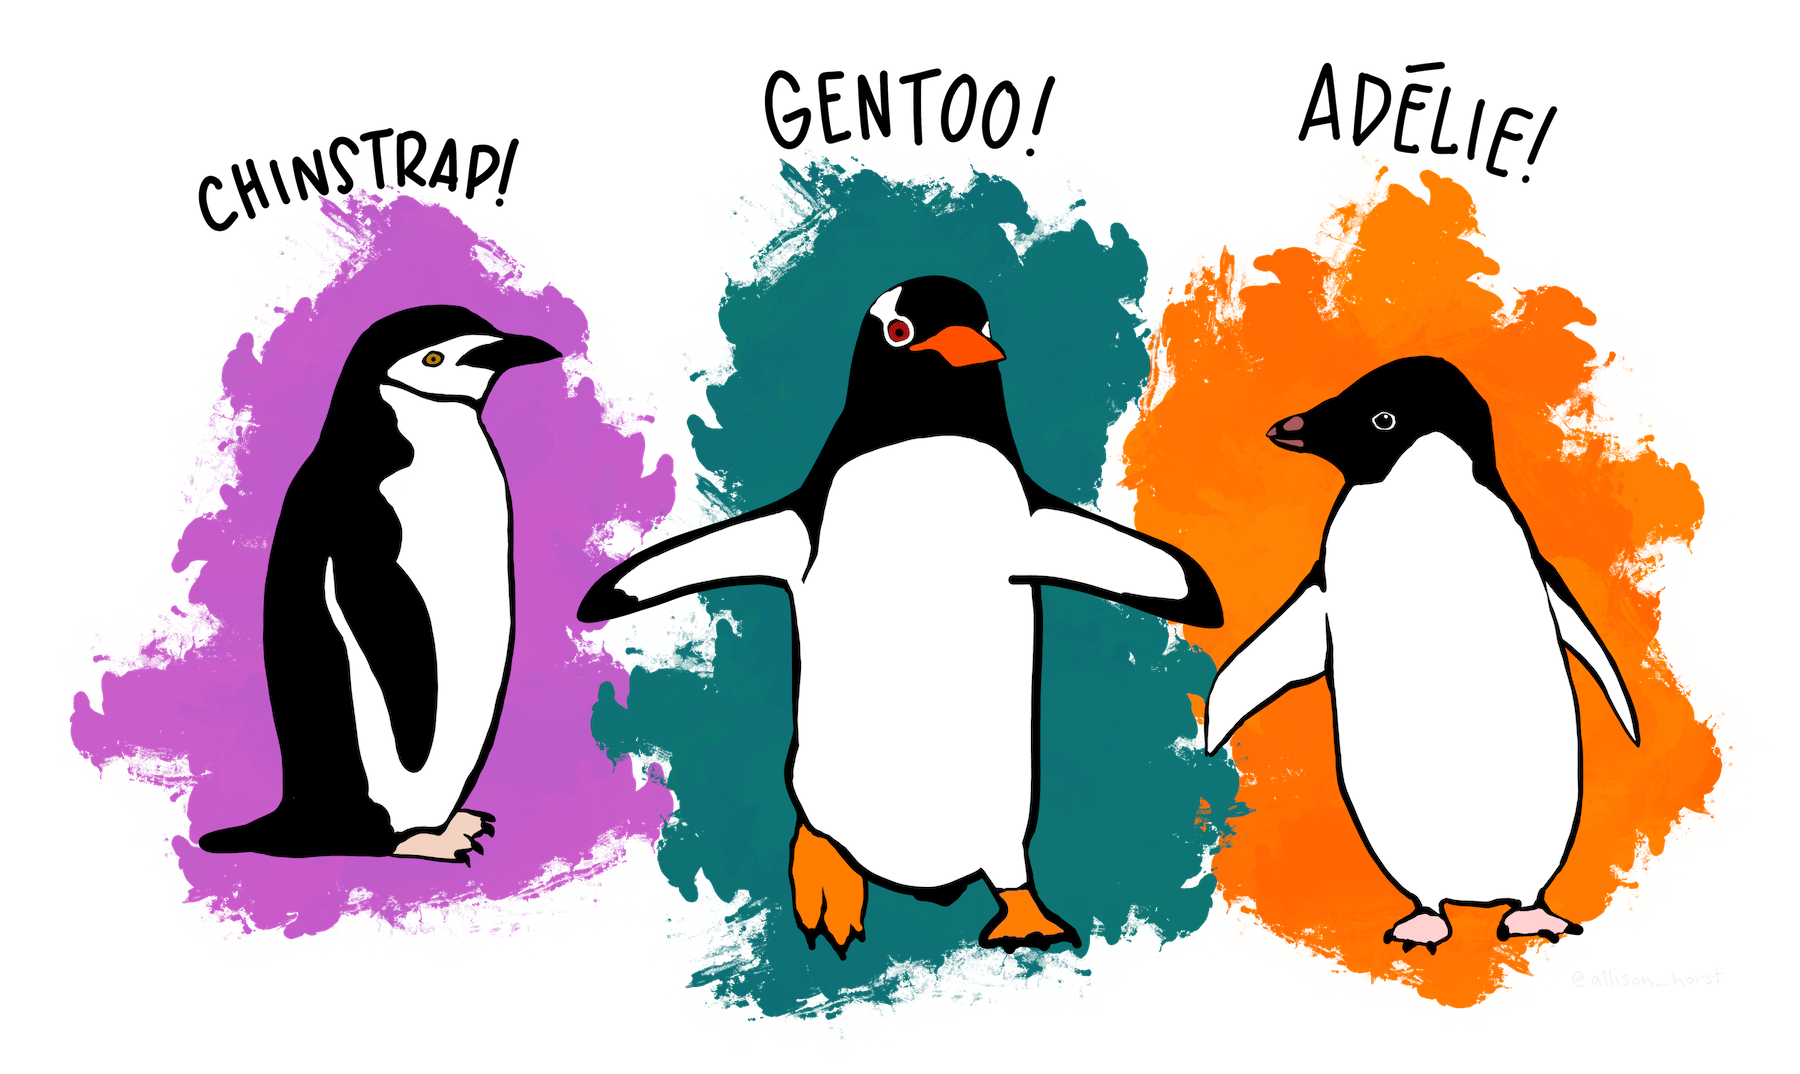
\includegraphics[width=0.5\linewidth]{images/lter_penguins} 

}

\caption{Happy coding}\label{fig:unnamed-chunk-9}
\end{figure}

\hypertarget{introduction-to-github-with-r}{%
\chapter{Introduction to github with R}\label{introduction-to-github-with-r}}

\hypertarget{practical-1}{%
\section{Practical}\label{practical-1}}

\hypertarget{context-1}{%
\subsection{Context}\label{context-1}}

We will configure Rstudio to work with our github account, then create a new project and start using \texttt{github}. To have some data I suggest to use the awesome \texttt{palmerpenguins} dataset 🐧.

\hypertarget{information-of-the-data}{%
\subsection{Information of the data}\label{information-of-the-data}}

These data have been collected and shared by \href{https://www.uaf.edu/cfos/people/faculty/detail/kristen-gorman.php}{Dr.~Kristen Gorman} and \href{https://pal.lternet.edu/}{Palmer Station, Antarctica LTER}.

The package was built by Drs Allison Horst and Alison Hill, check out the \href{https://allisonhorst.github.io/palmerpenguins/}{official website}.

The package \texttt{palmerpenguins} has two datasets.

\begin{Shaded}
\begin{Highlighting}[]
\KeywordTok{library}\NormalTok{(palmerpenguins)}
\end{Highlighting}
\end{Shaded}

The dataset \texttt{penguins} is a simplified version of the raw data; see \texttt{?penguins} for more info:

\begin{Shaded}
\begin{Highlighting}[]
\KeywordTok{head}\NormalTok{(penguins)}
\end{Highlighting}
\end{Shaded}

\begin{verbatim}
## # A tibble: 6 x 8
##   species island bill_length_mm bill_depth_mm flipper_length_~ body_mass_g sex  
##   <fct>   <fct>           <dbl>         <dbl>            <int>       <int> <fct>
## 1 Adelie  Torge~           39.1          18.7              181        3750 male 
## 2 Adelie  Torge~           39.5          17.4              186        3800 fema~
## 3 Adelie  Torge~           40.3          18                195        3250 fema~
## 4 Adelie  Torge~           NA            NA                 NA          NA <NA> 
## 5 Adelie  Torge~           36.7          19.3              193        3450 fema~
## 6 Adelie  Torge~           39.3          20.6              190        3650 male 
## # ... with 1 more variable: year <int>
\end{verbatim}

The other dataset \texttt{penguins\_raw} has the raw data; see \texttt{?penguins\_raw} for more info:

\begin{Shaded}
\begin{Highlighting}[]
\KeywordTok{head}\NormalTok{(penguins_raw)}
\end{Highlighting}
\end{Shaded}

\begin{verbatim}
## # A tibble: 6 x 17
##   studyName `Sample Number` Species Region Island Stage `Individual ID`
##   <chr>               <dbl> <chr>   <chr>  <chr>  <chr> <chr>          
## 1 PAL0708                 1 Adelie~ Anvers Torge~ Adul~ N1A1           
## 2 PAL0708                 2 Adelie~ Anvers Torge~ Adul~ N1A2           
## 3 PAL0708                 3 Adelie~ Anvers Torge~ Adul~ N2A1           
## 4 PAL0708                 4 Adelie~ Anvers Torge~ Adul~ N2A2           
## 5 PAL0708                 5 Adelie~ Anvers Torge~ Adul~ N3A1           
## 6 PAL0708                 6 Adelie~ Anvers Torge~ Adul~ N3A2           
## # ... with 10 more variables: `Clutch Completion` <chr>, `Date Egg` <date>,
## #   `Culmen Length (mm)` <dbl>, `Culmen Depth (mm)` <dbl>, `Flipper Length
## #   (mm)` <dbl>, `Body Mass (g)` <dbl>, Sex <chr>, `Delta 15 N (o/oo)` <dbl>,
## #   `Delta 13 C (o/oo)` <dbl>, Comments <chr>
\end{verbatim}

For this exercise, we're gonna use the \texttt{penguins} dataset.

\hypertarget{questions-1}{%
\subsection{Questions}\label{questions-1}}

\textbf{1)} Create a github acocunt if not done yet.

\textbf{2)} Configure Rstudio with your github account using the \texttt{usethis} package.

\textbf{3)} Store your GITHUB Personal Authorisation Token in your .Renviron file

\textbf{4)} Create a new R Markdown project, and create a new git repository

\textbf{5)} Create a new Rmarkdon document, in your project. Then save the file and stage it.

\textbf{6)} Create a new commit including the new file and push it to github (Check on github that it works).

\textbf{7)} Edit the file. Delete everything after line 12. Add a new section title, simple text and text in bold font. Then knit and compile.

\textbf{8)} Make a new commit (with a meaningful message), and push to github.

\textbf{9)} Create a new branch, and add a new section to the rmarkdown file in this branch. Whatever you want. I would suggest a graph of the data.

\textbf{10)} Creat a commit and push it to the branch.

\textbf{11)} On github, create a pull request to merge the 2 different branches.

\textbf{12)} Check and accep the pull request to merge the 2 branches.

You have successfully used all the essential tools of \texttt{git} 🎉 . You are really to explore 🕵 and discover its power 💪

\begin{figure}

{\centering 
\includegraphics[width=0.3\linewidth]{images/github_ninja} 

}

\caption{Happy git(hub)-ing}\label{fig:unnamed-chunk-10}
\end{figure}

\hypertarget{part-statistics}{%
\part{Statistics}\label{part-statistics}}

\hypertarget{refresher-on-glm}{%
\chapter{\texorpdfstring{Refresher on \texttt{glm}}{Refresher on glm}}\label{refresher-on-glm}}

\begin{Shaded}
\begin{Highlighting}[]
\NormalTok{m1 <-}\StringTok{ }\KeywordTok{glm}\NormalTok{(fish }\OperatorTok{~}\StringTok{ }\NormalTok{french_captain, }\DataTypeTok{data =}\NormalTok{ dads_joke, }\DataTypeTok{family =}\NormalTok{ poisson)}
\end{Highlighting}
\end{Shaded}

\hypertarget{introduction-to-linear-mixed-models}{%
\chapter{Introduction to linear mixed models}\label{introduction-to-linear-mixed-models}}

\hypertarget{practical-2}{%
\section{Practical}\label{practical-2}}

\hypertarget{overview}{%
\subsection{Overview}\label{overview}}

This practical is intended to get you started fitting some simple mixed models with so called \emph{random intercepts}. The tutorial is derived from one that accompanied the paper \citep{houslay_avoiding_2017}, ``\href{https://doi.org/10.1093/beheco/arx023}{Avoiding the misuse of BLUP in behavioral ecology}''. Here, you will be working through a simplified version in which I have taken more time to cover the basic mixed models and don't cover multivariate models which were really the main point of that paper. So if you find this material interesting don't worry we will go through a more advanced version of the original paper on multivariate models in \protect\hyperlink{to_be_written}{chapter XX}. The original version will be worth a work through to help you break into multivariate mixed models anyway! Here we will:

\begin{itemize}
\tightlist
\item
  Learn how to fit - and interpret the results of - a simple univariate mixed effect model
\item
  See how to add fixed and random effects to your model, and to test their significance in the normal frequentists sense
\end{itemize}

We are going to use the 📦 \texttt{lme4} \citep{R-lme4} which is widely used and great for simple mixed models. However, since, for philosophical reasons, \texttt{lme4} does not provide any p-values for either fixed or random effects, we are going to use the 📦 \texttt{lmerTest} \citep{R-lmerTest}, which add a bunch a nice goodies to \texttt{lme4} For slightly more complex models, including multivariate ones, generalised models, and random effects of things like shared space, pedigree, phylogeny I tend to use different 📦 like \texttt{MCMCglmm} \citep{MCMCglmm2010} (which is Bayesian, look at Jarrod Hadfield's excellent course notes \citep{R-MCMCglmm}) or ASReml-R \citep{R-asreml} (which is likelihood based/frequentist but sadly is not free).

\hypertarget{r-packages-needed}{%
\subsection{R packages needed}\label{r-packages-needed}}

First we load required libraries

\begin{Shaded}
\begin{Highlighting}[]
\KeywordTok{library}\NormalTok{(lmerTest)}
\KeywordTok{library}\NormalTok{(tidyverse)}
\KeywordTok{library}\NormalTok{(rptR)}
\end{Highlighting}
\end{Shaded}

\hypertarget{the-superb-wild-unicorns-of-the-scottish-highlands}{%
\subsection{The superb wild unicorns of the Scottish Highlands}\label{the-superb-wild-unicorns-of-the-scottish-highlands}}

Unicorns, a legendary animal and also symbol or Scotland, are frequently described as extremely wild woodland creature but also a symbol of purity and grace. Here is one of most accurate representation of the lengendary animal.

\begin{figure}

{\centering 
\includegraphics[width=0.5\linewidth]{images/unicorn} 

}

\caption{The superb unicorn of the Scottish Highlands}\label{fig:unnamed-chunk-12}
\end{figure}

Despite their image of purity and grace, unicorns (\emph{Unicornus legendaricus}) are raging fighter when it comes to compete for the best sweets you can find at the bottom of rainbows (unicorn favourite source of food).

We want to know:

\begin{itemize}
\tightlist
\item
  If aggressiveness differs among individuals
\item
  If aggressive behaviour is plastic (change with the environment)
\item
  If aggressive behaviour depends on body condition of focal animal
\end{itemize}

With respect to plasticity, we will focus on rival size as an `environment'. Common sense, and animal-contest theory, suggest a small animal would be wise not to escalate an aggressive contest against a larger, stronger rival. However, there are reports in the legendary beasty literature that they get more aggressive as rival size increases. Those reports are based on small sample sizes and uncontrolled field observations by foreigners Munro baggers enjoying their whisky after a long day in the hills.

\hypertarget{experimental-design}{%
\subsubsection{Experimental design}\label{experimental-design}}

Here, we have measured aggression in a population of wild unicorns. We brought some (n=80) individual into the lab, tagged them so they were individually identifiable, then repeatedly observed their aggression when presented with model `intruders' (animal care committe approved). There were three models; one of average unicorn (calculated as the population mean body length), one that was build to be 1 standard deviation below the population mean, and one that was 1 standard deviation above.

Data were collected on all individuals in two block of lab work. Within each block, each animal was tested 3 times, once against an `intruder' of each size. The test order in which each animal experienced the three instruder sizes was randomised in each block. The body size of all focal individuals was measured at the beginning of each block so we know that too (and have two separate measures per individual).

\hypertarget{looking-at-the-data}{%
\subsubsection{looking at the data}\label{looking-at-the-data}}

Let's load the data file \texttt{unicorns\_aggression.csv} in a R object named \texttt{unicorns} and make sure we understand what it contains

\begin{Shaded}
\begin{Highlighting}[]
\NormalTok{unicorns <-}\StringTok{ }\KeywordTok{read.csv}\NormalTok{(}\StringTok{"data/unicorns_aggression.csv"}\NormalTok{)}
\end{Highlighting}
\end{Shaded}

You can use \texttt{summary(unicorns)} to get an overview of the data and/or \texttt{str(unicorns)} to see the structure in the first few lines. This data frame has 6 variables:

\begin{Shaded}
\begin{Highlighting}[]
\KeywordTok{str}\NormalTok{(unicorns)}
\end{Highlighting}
\end{Shaded}

\begin{verbatim}
## 'data.frame':    480 obs. of  6 variables:
##  $ ID        : chr  "ID_1" "ID_1" "ID_1" "ID_1" ...
##  $ block     : num  -0.5 -0.5 -0.5 0.5 0.5 0.5 -0.5 -0.5 -0.5 0.5 ...
##  $ assay_rep : int  1 2 3 1 2 3 1 2 3 1 ...
##  $ opp_size  : int  -1 1 0 0 1 -1 1 -1 0 1 ...
##  $ aggression: num  7.02 10.67 10.22 8.95 10.51 ...
##  $ body_size : num  206 206 206 207 207 ...
\end{verbatim}

\begin{Shaded}
\begin{Highlighting}[]
\KeywordTok{summary}\NormalTok{(unicorns)}
\end{Highlighting}
\end{Shaded}

\begin{verbatim}
##       ID                block        assay_rep    opp_size    aggression    
##  Length:480         Min.   :-0.5   Min.   :1   Min.   :-1   Min.   : 5.900  
##  Class :character   1st Qu.:-0.5   1st Qu.:1   1st Qu.:-1   1st Qu.: 8.158  
##  Mode  :character   Median : 0.0   Median :2   Median : 0   Median : 8.950  
##                     Mean   : 0.0   Mean   :2   Mean   : 0   Mean   : 9.002  
##                     3rd Qu.: 0.5   3rd Qu.:3   3rd Qu.: 1   3rd Qu.: 9.822  
##                     Max.   : 0.5   Max.   :3   Max.   : 1   Max.   :12.170  
##    body_size    
##  Min.   :192.0  
##  1st Qu.:229.7  
##  Median :250.0  
##  Mean   :252.5  
##  3rd Qu.:272.0  
##  Max.   :345.2
\end{verbatim}

So the different columns in the data set are:

\begin{itemize}
\tightlist
\item
  Individual \textbf{ID}
\item
  Experimental \textbf{Block}, denoted for now as a continuous variable with possible values of -0.5 (first block) or +0.5 (second block)
\item
  Individual \textbf{body\_size}, as measured at the start of each block in kg
\item
  The repeat number for each behavioural test, \textbf{assay\_rep}
\item
  Opponent size (\textbf{opp\_size}), in standard deviations from the mean (i.e., -1,0,1)
\item
  \textbf{aggression}, our behavioural trait, measured 6 times in total per individual (2 blocks of 3 tests)
\end{itemize}

\emph{maybe add something on how to look at data structure closely using tables}

\hypertarget{do-unicorns-differ-in-aggressiveness-your-first-mixed-model}{%
\subsection{Do unicorns differ in aggressiveness? Your first mixed model}\label{do-unicorns-differ-in-aggressiveness-your-first-mixed-model}}

Fit a first mixed model with \texttt{lmer} that have only individual identity as a random effect and only a population mean.

Why, so simple? Because we simply want to partition variance around the mean into a component that among-individual variance and one that is within-individual variance.

A sensible researcher would probably take the time to do some exploratory data plots here. So let's write a mixed model. This one is going to have no fixed effects except the mean, and just one random effect - individual identity.

\begin{Shaded}
\begin{Highlighting}[]
\NormalTok{m_}\DecValTok{1}\NormalTok{ <-}\StringTok{ }\KeywordTok{lmer}\NormalTok{(aggression }\OperatorTok{~}\StringTok{ }\DecValTok{1} \OperatorTok{+}\StringTok{  }\NormalTok{(}\DecValTok{1} \OperatorTok{|}\StringTok{ }\NormalTok{ID), }\DataTypeTok{data =}\NormalTok{ unicorns)}
\end{Highlighting}
\end{Shaded}

\begin{verbatim}
## boundary (singular) fit: see ?isSingular
\end{verbatim}

There is a warning\ldots{} something about ``singularities''. Ignore that for a moment.

Now you need to get the model output. By that I just mean use \texttt{summary(model\_name)}.

\begin{Shaded}
\begin{Highlighting}[]
\KeywordTok{summary}\NormalTok{(m_}\DecValTok{1}\NormalTok{)}
\end{Highlighting}
\end{Shaded}

\begin{verbatim}
## Linear mixed model fit by REML. t-tests use Satterthwaite's method [
## lmerModLmerTest]
## Formula: aggression ~ 1 + (1 | ID)
##    Data: unicorns
## 
## REML criterion at convergence: 1503.7
## 
## Scaled residuals: 
##      Min       1Q   Median       3Q      Max 
## -2.68530 -0.73094 -0.04486  0.71048  2.74276 
## 
## Random effects:
##  Groups   Name        Variance Std.Dev.
##  ID       (Intercept) 0.000    0.000   
##  Residual             1.334    1.155   
## Number of obs: 480, groups:  ID, 80
## 
## Fixed effects:
##              Estimate Std. Error        df t value Pr(>|t|)    
## (Intercept)   9.00181    0.05272 479.00000   170.7   <2e-16 ***
## ---
## Signif. codes:  0 '***' 0.001 '**' 0.01 '*' 0.05 '.' 0.1 ' ' 1
## optimizer (nloptwrap) convergence code: 0 (OK)
## boundary (singular) fit: see ?isSingular
\end{verbatim}

In the summary you will find a table of fixed effects.

\begin{verbatim}
Fixed effects:
             Estimate Std. Error        df t value Pr(>|t|)    
(Intercept)   9.00181    0.05272 479.00000   170.7   <2e-16 ***
\end{verbatim}

The intercept (here the mean) is about 9 and is significantly \textgreater0 - fine, but not very interesting to us.

You will also find a random effect table that contains estimates of the among individual (ID) and residual variances.

\begin{verbatim}
Random effects:
 Groups   Name        Variance Std.Dev.
 ID       (Intercept) 0.000    0.000   
 Residual             1.334    1.155   
Number of obs: 480, groups:  ID, 80
\end{verbatim}

The among individual (ID) is estimated as zero. In fact this is what the cryptic warning was about: in most situations the idea of a random effect explaining less than zero variance is not sensible (strangely there are exception!). So by default the variance estimates are constrained to lie in positive parameter space. Here in trying to find the maximum likelihood solution for among-individual variance, our model has run up against this constraint.

\hypertarget{testing-for-random-effects}{%
\subsubsection{Testing for random effects}\label{testing-for-random-effects}}

We can test the statistical significance of the random effect using the \texttt{ranova()} command in \texttt{lmerTest}. This function is actually doing a \emph{likelihood ratio test} (LRT) of the random effect. The premise of which is that twice the difference in log-likelihood of the full and reduced (i.e.~with the random effect dropped) is itself distributed as \(\chi^2\)\$ with DF equal to the number of parameters dropped (here 1). Actually, there is a good argument that this is too conservative, but we can discuss that later. So let's do the LRT for the random effect using \texttt{ranova()}

\begin{Shaded}
\begin{Highlighting}[]
\KeywordTok{ranova}\NormalTok{(m_}\DecValTok{1}\NormalTok{)}
\end{Highlighting}
\end{Shaded}

\begin{verbatim}
## ANOVA-like table for random-effects: Single term deletions
## 
## Model:
## aggression ~ (1 | ID)
##          npar  logLik    AIC LRT Df Pr(>Chisq)
## <none>      3 -751.83 1509.7                  
## (1 | ID)    2 -751.83 1507.7   0  1          1
\end{verbatim}

There is apparently no among-individual variance in aggressiveness.

So this is a fairly rubbish and underwhelming model. Let's improve it.

\hypertarget{do-unicorns-differ-in-aggressiveness-a-better-mixed-model}{%
\subsection{Do unicorns differ in aggressiveness? A better mixed model}\label{do-unicorns-differ-in-aggressiveness-a-better-mixed-model}}

The answer we got from our first model is \textbf{not} wrong, it estimated the parameters we asked for and that might be informative or not and that might be representative or not of the true biology. Anyway all models are \textbf{wrong} but as models go this one is fairly rubbish. In fact we have explained no variation at all as we have no fixed effects (except the mean) and our random effect variance is zero. We woud have seen just how pointless this model was if we'd plotted it

\begin{Shaded}
\begin{Highlighting}[]
\KeywordTok{plot}\NormalTok{(m_}\DecValTok{1}\NormalTok{)}
\end{Highlighting}
\end{Shaded}

\begin{figure}
\centering
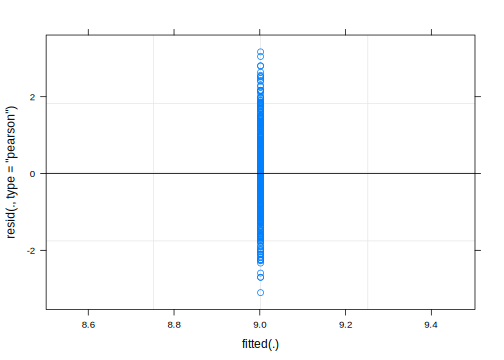
\includegraphics{BIO8940_book_files/figure-latex/mod1_plot-1.pdf}
\caption{(\#fig:mod1\_plot)Fitted values vs residuals for a simple mixed model of unicorn aggression}
\end{figure}

So we can probably do better at modelling the data, which may or may not change our view on whether there is any real variation among unicorns in aggressiveness.

For instance, we can (and should have started with) an initial plot of the phenotypic data against opponent size indicates to have a look at our prediction.

The code below uses the excellent 📦 \texttt{ggplot2} but the same figure can be done using base R code.

\begin{Shaded}
\begin{Highlighting}[]
\KeywordTok{ggplot}\NormalTok{(unicorns, }\KeywordTok{aes}\NormalTok{(}\DataTypeTok{x =}\NormalTok{ opp_size, }\DataTypeTok{y =}\NormalTok{ aggression)) }\OperatorTok{+}
\StringTok{  }\KeywordTok{geom_jitter}\NormalTok{(}
    \DataTypeTok{alpha =} \FloatTok{0.5}\NormalTok{,}
    \DataTypeTok{width =} \FloatTok{0.05}
\NormalTok{  ) }\OperatorTok{+}
\StringTok{  }\KeywordTok{scale_x_continuous}\NormalTok{(}\DataTypeTok{breaks =} \KeywordTok{c}\NormalTok{(}\OperatorTok{-}\DecValTok{1}\NormalTok{, }\DecValTok{0}\NormalTok{, }\DecValTok{1}\NormalTok{)) }\OperatorTok{+}
\StringTok{  }\KeywordTok{labs}\NormalTok{(}
    \DataTypeTok{x =} \StringTok{"Opponent size (SD)"}\NormalTok{,}
    \DataTypeTok{y =} \StringTok{"Aggression"}
\NormalTok{  ) }\OperatorTok{+}
\StringTok{  }\KeywordTok{theme_classic}\NormalTok{()}
\end{Highlighting}
\end{Shaded}

\begin{Shaded}
\begin{Highlighting}[]
\KeywordTok{ggplot}\NormalTok{(unicorns, }\KeywordTok{aes}\NormalTok{(}\DataTypeTok{x =}\NormalTok{ opp_size, }\DataTypeTok{y =}\NormalTok{ aggression)) }\OperatorTok{+}
\StringTok{  }\KeywordTok{geom_jitter}\NormalTok{(}
    \DataTypeTok{alpha =} \FloatTok{0.5}\NormalTok{,}
    \DataTypeTok{width =} \FloatTok{0.05}
\NormalTok{  ) }\OperatorTok{+}
\StringTok{  }\KeywordTok{scale_x_continuous}\NormalTok{(}\DataTypeTok{breaks =} \KeywordTok{c}\NormalTok{(}\OperatorTok{-}\DecValTok{1}\NormalTok{, }\DecValTok{0}\NormalTok{, }\DecValTok{1}\NormalTok{)) }\OperatorTok{+}
\StringTok{  }\KeywordTok{labs}\NormalTok{(}
    \DataTypeTok{x =} \StringTok{"Opponent size (SD)"}\NormalTok{,}
    \DataTypeTok{y =} \StringTok{"Aggression"}
\NormalTok{  ) }\OperatorTok{+}
\StringTok{  }\KeywordTok{theme_classic}\NormalTok{()}
\end{Highlighting}
\end{Shaded}

\begin{figure}

{\centering 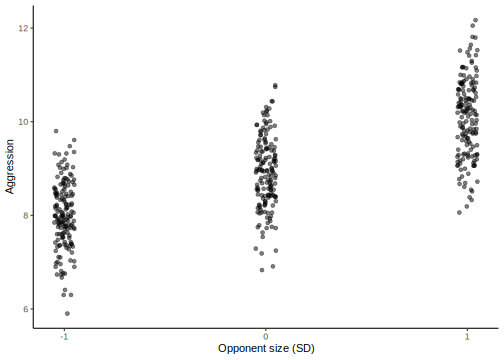
\includegraphics{BIO8940_book_files/figure-latex/rplotaggr-1} 

}

\caption{Unicorn aggressivity as a function of opponent size when fighting for sweets}\label{fig:rplotaggr}
\end{figure}

As predicted, there is a general increase in aggression with opponent size (points are lightly jittered on the x-axis to show the spread of data a little better)

You can see the same thing from a quick look at the population means for aggression at opponent size. Here we do it with the \texttt{kable} function that makes nice tables in \texttt{rmarkdown} documents.

\begin{Shaded}
\begin{Highlighting}[]
\NormalTok{unicorns }\OperatorTok
\StringTok{  }\KeywordTok{group_by}\NormalTok{(opp_size) }\OperatorTok
\StringTok{  }\KeywordTok{summarise}\NormalTok{(}\DataTypeTok{mean_aggr =} \KeywordTok{mean}\NormalTok{(aggression)) }\OperatorTok
\StringTok{  }\NormalTok{knitr}\OperatorTok{::}\KeywordTok{kable}\NormalTok{(}\DataTypeTok{digits =} \DecValTok{2}\NormalTok{)}
\end{Highlighting}
\end{Shaded}

\begin{tabular}{r}
\hline
mean\_aggr\\
\hline
9\\
\hline
\end{tabular}

So, there does appear to be plasticity of aggression with changing size of the model opponent. But other things may explain variation in aggressiveness too - what about block for instance? Block effects may not be the subject of any biologically interesting hypotheses, but accounting for any differences between blocks could remove noise.

There may also be systematic change in behaviour as an individual experiences more repeat observations (i.e.~exposure to the model). Do they get sensitised or habituated to the model intruder for example?

So let's run a mixed model with the same random effect of individual, but with a fixed effects of opponent size (our predictor of interest) and experimental block.

\begin{Shaded}
\begin{Highlighting}[]
\NormalTok{m_}\DecValTok{2}\NormalTok{ <-}\StringTok{ }\KeywordTok{lmer}\NormalTok{(aggression }\OperatorTok{~}\StringTok{ }\NormalTok{opp_size  }\OperatorTok{+}\StringTok{ }\NormalTok{block }\OperatorTok{+}\StringTok{ }\NormalTok{(}\DecValTok{1} \OperatorTok{|}\StringTok{ }\NormalTok{ID), }\DataTypeTok{data =}\NormalTok{ unicorns)}
\end{Highlighting}
\end{Shaded}

\hypertarget{diagnostic-plots}{%
\subsubsection{Diagnostic plots}\label{diagnostic-plots}}

Run a few diagnostic plots before we look at the answers. In diagnostic plots, we want to check the condition of applications of the linear mixed model which are the same 4 as the linear model plus 2 extra:

\begin{enumerate}
\def\labelenumi{\arabic{enumi}.}
\item
  Linearity of the relation between covariates and the response
\item
  No error on measurement of covariates
\item
  Residual have a Gaussian distribution
\item
  Homoscedasticty (variance of residuals is constant across covariates)
\item
  Random effects have a Gaussian distribution
\item
  Residual variance is constant across all levels of a random effect
\end{enumerate}

This is checked with:

\begin{enumerate}
\def\labelenumi{\arabic{enumi}.}
\tightlist
\item
  done with data exploration graph (i.e.~just plot the data see if it is linear)

  \begin{itemize}
  \tightlist
  \item
    see previous graph
  \end{itemize}
\item
  assumed to be correct if measurement error is lower than 10\% of variance in the variable

  \begin{itemize}
  \tightlist
  \item
    I know this sounds pretty bad
  \end{itemize}
\item
  using quantile-quantile plot or histogram of residuals
\end{enumerate}

\begin{Shaded}
\begin{Highlighting}[]
\KeywordTok{par}\NormalTok{(}\DataTypeTok{mfrow =} \KeywordTok{c}\NormalTok{(}\DecValTok{1}\NormalTok{, }\DecValTok{2}\NormalTok{)) }\CommentTok{# multiple graphs in a window}
\KeywordTok{qqnorm}\NormalTok{(}\KeywordTok{residuals}\NormalTok{(m_}\DecValTok{2}\NormalTok{)) }\CommentTok{# a q-q plot}
\KeywordTok{qqline}\NormalTok{(}\KeywordTok{residuals}\NormalTok{(m_}\DecValTok{2}\NormalTok{))}
\KeywordTok{hist}\NormalTok{(}\KeywordTok{resid}\NormalTok{(m_}\DecValTok{2}\NormalTok{)) }\CommentTok{# are the residuals roughly Gaussian?}
\end{Highlighting}
\end{Shaded}

\begin{figure}
\centering
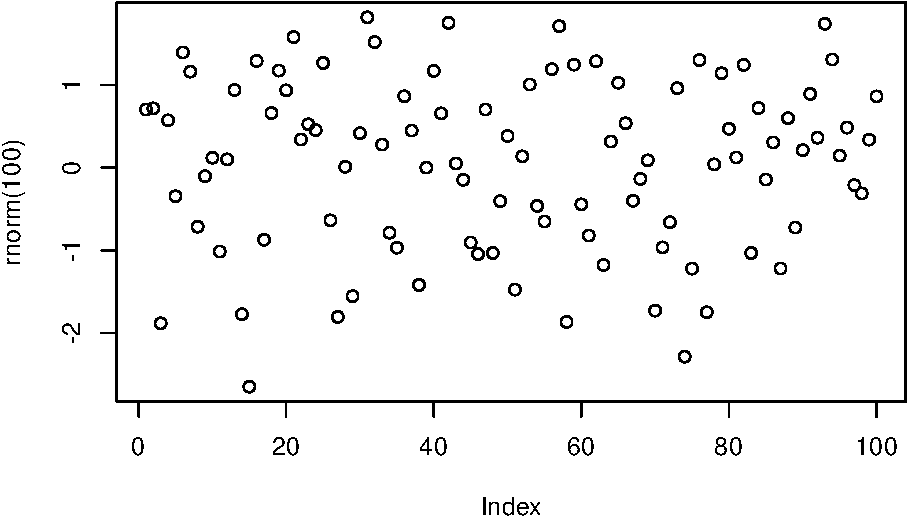
\includegraphics{BIO8940_book_files/figure-latex/unnamed-chunk-14-1.pdf}
\caption{\label{fig:unnamed-chunk-14}Checking residuals have Gaussian distribution}
\end{figure}

\begin{enumerate}
\def\labelenumi{\arabic{enumi}.}
\setcounter{enumi}{3}
\tightlist
\item
  using plot of residuals by fitted values
\end{enumerate}

\begin{Shaded}
\begin{Highlighting}[]
\KeywordTok{plot}\NormalTok{(m_}\DecValTok{2}\NormalTok{)}
\end{Highlighting}
\end{Shaded}

\begin{figure}
\centering
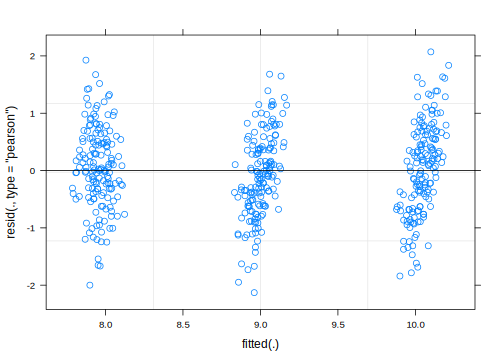
\includegraphics{BIO8940_book_files/figure-latex/unnamed-chunk-15-1.pdf}
\caption{\label{fig:unnamed-chunk-15}Residuals by fitted values for model m\_2 to check homoscedasticity}
\end{figure}

\begin{enumerate}
\def\labelenumi{\arabic{enumi}.}
\setcounter{enumi}{4}
\tightlist
\item
  histogram of the predictions for the random effects (BLUPs)
\end{enumerate}

\begin{Shaded}
\begin{Highlighting}[]
\CommentTok{# extracting blups}
\NormalTok{r1 <-}\StringTok{ }\KeywordTok{as.data.frame}\NormalTok{(}\KeywordTok{ranef}\NormalTok{(m_}\DecValTok{2}\NormalTok{, }\DataTypeTok{condVar =} \OtherTok{TRUE}\NormalTok{))}

\KeywordTok{par}\NormalTok{(}\DataTypeTok{mfrow =} \KeywordTok{c}\NormalTok{(}\DecValTok{1}\NormalTok{, }\DecValTok{2}\NormalTok{))}
\KeywordTok{hist}\NormalTok{(r1}\OperatorTok{$}\NormalTok{condval)}
\KeywordTok{qqnorm}\NormalTok{(r1}\OperatorTok{$}\NormalTok{condval)}
\KeywordTok{qqline}\NormalTok{(r1}\OperatorTok{$}\NormalTok{condval)}
\end{Highlighting}
\end{Shaded}

\begin{figure}
\centering
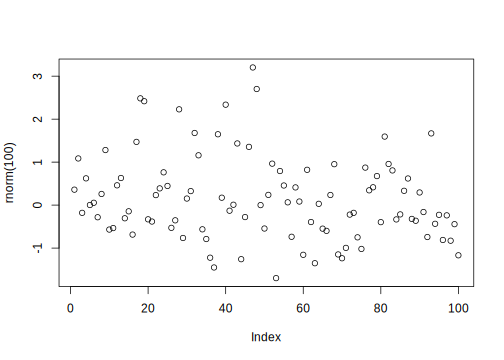
\includegraphics{BIO8940_book_files/figure-latex/unnamed-chunk-16-1.pdf}
\caption{\label{fig:unnamed-chunk-16}Checking random effects are gaussian}
\end{figure}

\begin{enumerate}
\def\labelenumi{\arabic{enumi}.}
\setcounter{enumi}{5}
\tightlist
\item
  plotting the sorted BLUPs with their errors
\end{enumerate}

\begin{Shaded}
\begin{Highlighting}[]
\NormalTok{r1 <-}\StringTok{ }\NormalTok{r1[}\KeywordTok{order}\NormalTok{(r1}\OperatorTok{$}\NormalTok{condval), ] }\CommentTok{# sorting the BLUPs}
\KeywordTok{ggplot}\NormalTok{(r1, }\KeywordTok{aes}\NormalTok{(}\DataTypeTok{y =}\NormalTok{ grp, }\DataTypeTok{x =}\NormalTok{ condval)) }\OperatorTok{+}
\StringTok{  }\KeywordTok{geom_point}\NormalTok{() }\OperatorTok{+}
\StringTok{  }\KeywordTok{geom_pointrange}\NormalTok{(}
    \KeywordTok{aes}\NormalTok{(}\DataTypeTok{xmin =}\NormalTok{ condval }\OperatorTok{-}\StringTok{ }\NormalTok{condsd }\OperatorTok{*}\StringTok{ }\FloatTok{1.96}\NormalTok{, }\DataTypeTok{xmax =}\NormalTok{ condval }\OperatorTok{+}\StringTok{ }\NormalTok{condsd }\OperatorTok{*}\StringTok{ }\FloatTok{1.96}\NormalTok{)}
\NormalTok{  ) }\OperatorTok{+}
\StringTok{  }\KeywordTok{geom_vline}\NormalTok{(}\KeywordTok{aes}\NormalTok{(}\DataTypeTok{xintercept =} \DecValTok{0}\NormalTok{, }\DataTypeTok{color =} \StringTok{"red"}\NormalTok{)) }\OperatorTok{+}
\StringTok{  }\KeywordTok{theme_classic}\NormalTok{() }\OperatorTok{+}
\StringTok{  }\KeywordTok{theme}\NormalTok{(}\DataTypeTok{legend.position =} \StringTok{"none"}\NormalTok{)}
\end{Highlighting}
\end{Shaded}

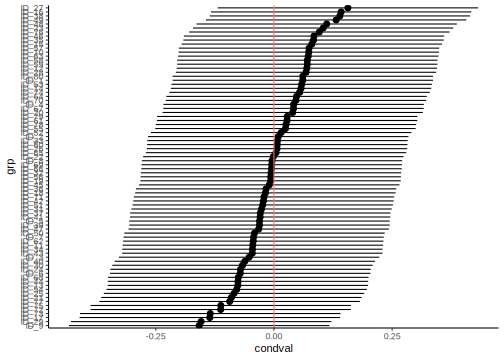
\includegraphics{BIO8940_book_files/figure-latex/mod2_plots-1.pdf}

\hypertarget{inferences}{%
\subsubsection{Inferences}\label{inferences}}

\textbf{Now summarise this model. We will pause here for you to think about and discuss a few things:}
* What can you take from the fixed effect table?
* How do you interpret the intercept now that there are other effects in the model?
* What would happen if we scaled our fixed covariates differently? Why?

\begin{Shaded}
\begin{Highlighting}[]
\KeywordTok{summary}\NormalTok{(m_}\DecValTok{2}\NormalTok{)}
\end{Highlighting}
\end{Shaded}

\begin{verbatim}
## Linear mixed model fit by REML. t-tests use Satterthwaite's method [
## lmerModLmerTest]
## Formula: aggression ~ opp_size + block + (1 | ID)
##    Data: unicorns
## 
## REML criterion at convergence: 1129.9
## 
## Scaled residuals: 
##      Min       1Q   Median       3Q      Max 
## -2.79296 -0.64761  0.00155  0.67586  2.71456 
## 
## Random effects:
##  Groups   Name        Variance Std.Dev.
##  ID       (Intercept) 0.02478  0.1574  
##  Residual             0.58166  0.7627  
## Number of obs: 480, groups:  ID, 80
## 
## Fixed effects:
##              Estimate Std. Error        df t value Pr(>|t|)    
## (Intercept)   9.00181    0.03901  79.00000 230.778   <2e-16 ***
## opp_size      1.04562    0.04263 398.00000  24.525   <2e-16 ***
## block        -0.02179    0.06962 398.00000  -0.313    0.754    
## ---
## Signif. codes:  0 '***' 0.001 '**' 0.01 '*' 0.05 '.' 0.1 ' ' 1
## 
## Correlation of Fixed Effects:
##          (Intr) opp_sz
## opp_size 0.000        
## block    0.000  0.000
\end{verbatim}

\begin{rmdcode}
\textbf{Try tweaking the fixed part of your model:}

\begin{itemize}
\tightlist
\item
  What happens if you add more fixed effects? Try it!
\item
  Could focal body size also matter? If so, should you rescale before adding it to the model?
\item
  Should you add interactions (e.g.~block:opp\_size)?
\item
  Should you drop non-significant fixed effects?
\end{itemize}
\end{rmdcode}

\begin{rmdcode}
\textbf{Having changed the fixed part of your model, do the variance estimates change at all?}

\begin{itemize}
\tightlist
\item
  Is among-individual variance always estimated as zero regardless of fixed effects?
\item
  Is among-individual variance significant with some fixed effets structures but not others?
\end{itemize}
\end{rmdcode}

\hypertarget{what-is-the-repeatability}{%
\subsection{What is the repeatability?}\label{what-is-the-repeatability}}

As a reminder, repeatability is the proportion of variance explained by a random effect and it is estimate as the ratio of the variance associated to a random effect by the total variance, or the sum of the residual variance and the different variance compoentn associated with the random effects.
In our first model among-individual variance was zero, so R was zero. If we have a different model of aggression and get a non-zero value of the random effect variance, we can obviously calculate a repeatability estimate (R). So we are all working from the same starting point, let's all stick with a common set of fixed effects from here on:

\begin{Shaded}
\begin{Highlighting}[]
\NormalTok{m_}\DecValTok{3}\NormalTok{ <-}\StringTok{ }\KeywordTok{lmer}\NormalTok{(}
\NormalTok{  aggression }\OperatorTok{~}\StringTok{ }\NormalTok{opp_size }\OperatorTok{+}\StringTok{ }\KeywordTok{scale}\NormalTok{(body_size, }\DataTypeTok{center =} \OtherTok{TRUE}\NormalTok{, }\DataTypeTok{scale =} \OtherTok{TRUE}\NormalTok{)}
              \OperatorTok{+}\StringTok{ }\KeywordTok{scale}\NormalTok{(assay_rep, }\DataTypeTok{scale =} \OtherTok{FALSE}\NormalTok{) }\OperatorTok{+}\StringTok{ }\NormalTok{block}
              \OperatorTok{+}\StringTok{ }\NormalTok{(}\DecValTok{1} \OperatorTok{|}\StringTok{ }\NormalTok{ID),}
  \DataTypeTok{data =}\NormalTok{ unicorns)}
\KeywordTok{summary}\NormalTok{(m_}\DecValTok{3}\NormalTok{)}
\end{Highlighting}
\end{Shaded}

\begin{verbatim}
## Linear mixed model fit by REML. t-tests use Satterthwaite's method [
## lmerModLmerTest]
## Formula: 
## aggression ~ opp_size + scale(body_size, center = TRUE, scale = TRUE) +  
##     scale(assay_rep, scale = FALSE) + block + (1 | ID)
##    Data: unicorns
## 
## REML criterion at convergence: 1136.5
## 
## Scaled residuals: 
##      Min       1Q   Median       3Q      Max 
## -2.85473 -0.62831  0.02545  0.68998  2.74064 
## 
## Random effects:
##  Groups   Name        Variance Std.Dev.
##  ID       (Intercept) 0.02538  0.1593  
##  Residual             0.58048  0.7619  
## Number of obs: 480, groups:  ID, 80
## 
## Fixed effects:
##                                                Estimate Std. Error        df
## (Intercept)                                     9.00181    0.03907  78.07315
## opp_size                                        1.05141    0.04281 396.99857
## scale(body_size, center = TRUE, scale = TRUE)   0.03310    0.03896  84.21144
## scale(assay_rep, scale = FALSE)                -0.05783    0.04281 396.99857
## block                                          -0.02166    0.06955 397.00209
##                                               t value Pr(>|t|)    
## (Intercept)                                   230.395   <2e-16 ***
## opp_size                                       24.562   <2e-16 ***
## scale(body_size, center = TRUE, scale = TRUE)   0.850    0.398    
## scale(assay_rep, scale = FALSE)                -1.351    0.177    
## block                                          -0.311    0.756    
## ---
## Signif. codes:  0 '***' 0.001 '**' 0.01 '*' 0.05 '.' 0.1 ' ' 1
## 
## Correlation of Fixed Effects:
##             (Intr) opp_sz sc=Ts=T s(_s=F
## opp_size     0.000                      
## s(_,c=TRs=T  0.000  0.000               
## s(_,s=FALSE  0.000 -0.100  0.000        
## block        0.000  0.000  0.002   0.000
\end{verbatim}

So we'd probably calculate R using the individual and residual variance simply as:

\begin{Shaded}
\begin{Highlighting}[]
\FloatTok{0.02538} \OperatorTok{/}\StringTok{ }\NormalTok{(}\FloatTok{0.02538} \OperatorTok{+}\StringTok{ }\FloatTok{0.58048}\NormalTok{)}
\end{Highlighting}
\end{Shaded}

\begin{verbatim}
## [1] 0.04189087
\end{verbatim}

\begin{rmdcode}
Do you see where I took the numbers ?
\end{rmdcode}

We can use some more fancy coding to extract the estimates and plugged them in a formula to estimate the repeatbility

\begin{Shaded}
\begin{Highlighting}[]
\NormalTok{v_id <-}\StringTok{ }\KeywordTok{VarCorr}\NormalTok{(m_}\DecValTok{3}\NormalTok{)}\OperatorTok{$}\NormalTok{ID[}\DecValTok{1}\NormalTok{, }\DecValTok{1}\NormalTok{]}
\NormalTok{v_r <-}\StringTok{ }\KeywordTok{attr}\NormalTok{(}\KeywordTok{VarCorr}\NormalTok{(m_}\DecValTok{3}\NormalTok{), }\StringTok{"sc"}\NormalTok{)}\OperatorTok{^}\DecValTok{2}
\NormalTok{r_man <-}\StringTok{ }\NormalTok{v_id }\OperatorTok{/}\StringTok{ }\NormalTok{(v_id }\OperatorTok{+}\StringTok{ }\NormalTok{v_r)}
\NormalTok{r_man}
\end{Highlighting}
\end{Shaded}

\begin{verbatim}
## [1] 0.04188879
\end{verbatim}

Which yields an estimate of approximately R=4\%. Strictly speaking we should make clear this a \textbf{conditional repeatability} estimate.

Conditional on what you might ask\ldots{} on the fixed effects in your model. So our best estimate of 4\% refers to the proportion of variance in aggressiveness \emph{not explained by fixed effects} that is explained by individual identity. This isn't much and still won't be significant, but illustrates the point that conditional repeatabilities often have a tendency to go up as people explain more of the residual variance by adding fixed effects. This is fine and proper, but can mislead the unwary reader.
It also means that decisions about which fixed effects to include in your model need to be based on how you want to interpret R not just on, for instance, whether fixed effects are deemed significant.

\hypertarget{a-quick-note-on-uncertainty}{%
\subsection{A quick note on uncertainty}\label{a-quick-note-on-uncertainty}}

Using \texttt{lmer} in the 📦 \texttt{lme4} 📦 there isn't a really simple way to put some measure of uncertainty (SE or CI) on derived parameters like repeatabilities. This is a bit annoying. Such things are more easily done with other mixed model 📦 like \texttt{MCMCglmm} and \texttt{asreml} which are a bit more specialist. If you are using \texttt{lmer} for models you want to publish then you could look into the 📦 \texttt{rptR} \citep{R-rptR}. This acts as a `wrapper' for \texttt{lmer} models and adds some nice functionality including options to boostrap confidence intervals. Regardless, of how you do it, if you want to put a repeatability in one of your papers as a key result - it really should be accompanied by a measure of uncertainty just like any other effect size estimate.

Here I am estimating the repeatability and using bootstrap to estimate a confidence interval and a probability associated with the repeatability with the \texttt{rptR} 📦. For more information about the use of the package and the theory behind it suggest the excellent paper associated with the package \citep{rptR2017}

\begin{Shaded}
\begin{Highlighting}[]
\NormalTok{r_rpt <-}\StringTok{ }\KeywordTok{rptGaussian}\NormalTok{(}
\NormalTok{  aggression }\OperatorTok{~}\StringTok{ }\NormalTok{opp_size }\OperatorTok{+}\StringTok{ }\NormalTok{block }\OperatorTok{+}\StringTok{ }\NormalTok{(}\DecValTok{1} \OperatorTok{|}\StringTok{ }\NormalTok{ID),}
  \DataTypeTok{grname =} \StringTok{"ID"}\NormalTok{, }\DataTypeTok{data =}\NormalTok{ unicorns)}
\end{Highlighting}
\end{Shaded}

\begin{verbatim}
## Bootstrap Progress:
\end{verbatim}

\begin{Shaded}
\begin{Highlighting}[]
\NormalTok{r_rpt}
\end{Highlighting}
\end{Shaded}

\begin{verbatim}
## 
## 
## Repeatability estimation using the lmm method 
## 
## Repeatability for ID
## R  = 0.041
## SE = 0.031
## CI = [0, 0.112]
## P  = 0.0966 [LRT]
##      NA [Permutation]
\end{verbatim}

\hypertarget{an-easy-way-to-mess-up-your-mixed-models}{%
\subsection{An easy way to mess up your mixed models}\label{an-easy-way-to-mess-up-your-mixed-models}}

We will try some more advanced mixed models in a moment to explore plasticity in aggressiveness a bit more. First let's quickly look for among-individual variance in focal body size. Why not? We have the data handy, everyone says morphological traits are very repeatable and - lets be honest - who wouldn't like to see a small P value after striking out with aggressiveness.

Include a random effect of ID as before and maybe a fixed effect of block, just to see if the beasties were growing a bit between data collection periods.

\begin{Shaded}
\begin{Highlighting}[]
\NormalTok{lmer_size <-}\StringTok{ }\KeywordTok{lmer}\NormalTok{(body_size }\OperatorTok{~}\StringTok{ }\NormalTok{block }\OperatorTok{+}\StringTok{ }\NormalTok{(}\DecValTok{1} \OperatorTok{|}\StringTok{ }\NormalTok{ID),}
                \DataTypeTok{data =}\NormalTok{ unicorns)}
\end{Highlighting}
\end{Shaded}

Summarise and test the random effect.

\begin{Shaded}
\begin{Highlighting}[]
\KeywordTok{summary}\NormalTok{(lmer_size)}
\end{Highlighting}
\end{Shaded}

\begin{verbatim}
## Linear mixed model fit by REML. t-tests use Satterthwaite's method [
## lmerModLmerTest]
## Formula: body_size ~ block + (1 | ID)
##    Data: unicorns
## 
## REML criterion at convergence: 3460.7
## 
## Scaled residuals: 
##      Min       1Q   Median       3Q      Max 
## -1.80452 -0.71319  0.00718  0.70280  1.81747 
## 
## Random effects:
##  Groups   Name        Variance Std.Dev.
##  ID       (Intercept) 936.01   30.594  
##  Residual              34.32    5.858  
## Number of obs: 480, groups:  ID, 80
## 
## Fixed effects:
##             Estimate Std. Error       df t value Pr(>|t|)    
## (Intercept) 252.5031     3.4310  79.0000  73.595   <2e-16 ***
## block        -0.1188     0.5348 399.0000  -0.222    0.824    
## ---
## Signif. codes:  0 '***' 0.001 '**' 0.01 '*' 0.05 '.' 0.1 ' ' 1
## 
## Correlation of Fixed Effects:
##       (Intr)
## block 0.000
\end{verbatim}

\begin{Shaded}
\begin{Highlighting}[]
\KeywordTok{ranova}\NormalTok{(lmer_size)}
\end{Highlighting}
\end{Shaded}

\begin{verbatim}
## ANOVA-like table for random-effects: Single term deletions
## 
## Model:
## body_size ~ block + (1 | ID)
##          npar  logLik    AIC    LRT Df Pr(>Chisq)    
## <none>      4 -1730.4 3468.7                         
## (1 | ID)    3 -2325.6 4657.1 1190.4  1  < 2.2e-16 ***
## ---
## Signif. codes:  0 '***' 0.001 '**' 0.01 '*' 0.05 '.' 0.1 ' ' 1
\end{verbatim}

\begin{rmdcode}
\textbf{What might you conclude, and why would this be foolish?}
\end{rmdcode}

Hopefully you spotted the problem here. You have fed in a data set with 6 records per individual (with 2 sets of 3 identical values per unicorns), when you know size was only measured twice in reality. This means you'd expect to get a (potentially very) upwardly biased estimate of R and a (potentially very) downwardly biased P value when testing among-individual variance.

\begin{rmdcode}
\textbf{How can we do it properly?}
\end{rmdcode}

We can prune the data to the two actual observations per unicorns by just selecting the first assay in each block.

\begin{Shaded}
\begin{Highlighting}[]
\NormalTok{unicorns2 <-}\StringTok{ }\NormalTok{unicorns[unicorns}\OperatorTok{$}\NormalTok{assay_rep }\OperatorTok{==}\StringTok{ }\DecValTok{1}\NormalTok{, ]}

\NormalTok{lmer_size2 <-}\StringTok{ }\KeywordTok{lmer}\NormalTok{(body_size }\OperatorTok{~}\StringTok{   }\NormalTok{block }\OperatorTok{+}\StringTok{  }\NormalTok{(}\DecValTok{1} \OperatorTok{|}\StringTok{ }\NormalTok{ID),}
                \DataTypeTok{data =}\NormalTok{ unicorns2)}
\KeywordTok{summary}\NormalTok{(lmer_size2)}
\end{Highlighting}
\end{Shaded}

\begin{verbatim}
## Linear mixed model fit by REML. t-tests use Satterthwaite's method [
## lmerModLmerTest]
## Formula: body_size ~ block + (1 | ID)
##    Data: unicorns2
## 
## REML criterion at convergence: 1373.4
## 
## Scaled residuals: 
##      Min       1Q   Median       3Q      Max 
## -1.54633 -0.56198  0.01319  0.56094  1.42095 
## 
## Random effects:
##  Groups   Name        Variance Std.Dev.
##  ID       (Intercept) 912.84   30.213  
##  Residual              57.78    7.601  
## Number of obs: 160, groups:  ID, 80
## 
## Fixed effects:
##             Estimate Std. Error       df t value Pr(>|t|)    
## (Intercept) 252.5031     3.4310  79.0000  73.595   <2e-16 ***
## block        -0.1188     1.2019  79.0000  -0.099    0.922    
## ---
## Signif. codes:  0 '***' 0.001 '**' 0.01 '*' 0.05 '.' 0.1 ' ' 1
## 
## Correlation of Fixed Effects:
##       (Intr)
## block 0.000
\end{verbatim}

\begin{Shaded}
\begin{Highlighting}[]
\KeywordTok{ranova}\NormalTok{(lmer_size2)}
\end{Highlighting}
\end{Shaded}

\begin{verbatim}
## ANOVA-like table for random-effects: Single term deletions
## 
## Model:
## body_size ~ block + (1 | ID)
##          npar  logLik    AIC    LRT Df Pr(>Chisq)    
## <none>      4 -686.68 1381.3                         
## (1 | ID)    3 -771.93 1549.9 170.51  1  < 2.2e-16 ***
## ---
## Signif. codes:  0 '***' 0.001 '**' 0.01 '*' 0.05 '.' 0.1 ' ' 1
\end{verbatim}

Summarise and test your random effect and you'll see the qualitative conclusions will actually be very similar using the pruned data set. Of course this won't generallty but be true, so just be careful. Mixed models are intended to help you model repeated measures data with non-independence, but they won't get you out of trouble if you mis-represent the true structure of observations on your dependent variable.

\hypertarget{happy-mixed-modelling}{%
\subsection{Happy mixed-modelling}\label{happy-mixed-modelling}}

\begin{figure}

{\centering 
\includegraphics[width=0.2\linewidth]{images/unicorn} 

}

\caption{The superb unicorn}\label{fig:unnamed-chunk-26}
\end{figure}

\hypertarget{introduction-to-glmm}{%
\chapter{\texorpdfstring{Introduction to \texttt{GLMM}}{Introduction to GLMM}}\label{introduction-to-glmm}}

\hypertarget{practical-3}{%
\section{Practical}\label{practical-3}}

Spatial variation in nutrient availability and herbivory is likely to cause pop-ulation differentiation and maintain genetic diversity in plant populations.Here we measure the extent to which mouse-ear cress (Arabidopsis thaliana)exhibits population and genotypic variation in their responses to these im-portant environmental factors. We are particularly interested in whetherthese populations exhibit nutrient mediated compensation, where higher nutrient levels allow genotypes to better tolerate herbivory (Banta et al.,2010). We use GLMMs to estimate the effect of nutrient levels, simulated hebivory, and their interaction on fruit production in Arabidopsis thaliana(fixed effects), and the extent to which populations vary in their responses(random effects, or variance components)

\hypertarget{packages-and-functions}{%
\subsection{Packages and functions}\label{packages-and-functions}}

You need to download the ``glmm\_funs.R'' script for some functions used in the Practical

\begin{Shaded}
\begin{Highlighting}[]
\KeywordTok{library}\NormalTok{(lme4)}
\KeywordTok{library}\NormalTok{(plyr)}
\KeywordTok{library}\NormalTok{(tidyverse)}
\KeywordTok{library}\NormalTok{(patchwork)}
\KeywordTok{library}\NormalTok{(lattice)}
\KeywordTok{source}\NormalTok{(}\StringTok{"data/glmm_funs.R"}\NormalTok{)}
\end{Highlighting}
\end{Shaded}

\hypertarget{the-data-set}{%
\subsection{The data set}\label{the-data-set}}

In this data set, the response variable is the number of fruits (i.e.~seedcapsules) per plant. The number of fruits produced by an individual plant(the experimental unit) was hypothesized to be a function of fixed effects,including nutrient levels (low vs.~high), simulated herbivory (none vs.~apicalmeristem damage), region (Sweden, Netherlands, Spain), and interactionsamong these. Fruit number was also a function of random effects including both the population and individual genotype. Because Arabidopsis is highlyselfing, seeds of a single individual served as replicates of that individual.There were also nuisance variables, including the placement of the plantin the greenhouse, and the method used to germinate seeds. These were estimated as fixed effects but interactions were excluded.

\begin{itemize}
\tightlist
\item
  \texttt{X} observation number (we will use this observation number later, when we are accounting for overdispersion)
\item
  \texttt{reg} a factor for region (Netherlands, Spain, Sweden).
\item
  \texttt{popu} a factor with a level for each population.
\item
  \texttt{gen} a factor with a level for each genotype.
\item
  \texttt{rack} a nuisance factor for one of two greenhouse racks.
\item
  \texttt{nutrient} a factor with levels for minimal or additional nutrients.
\item
  \texttt{amd} a factor with levels for no damage or simulated herbivory (apical meristem damage; we will sometimes refer to this as ``clipping'')
\item
  \texttt{status} a nuisance factor for germination method.
\item
  \texttt{total.fruits} the response; an integer count of the number of fruits perplant.
\end{itemize}

\hypertarget{specifying-fixed-and-random-effects}{%
\subsection{Specifying fixed and random Effects}\label{specifying-fixed-and-random-effects}}

Here we need to select a realistic full model, based on the scientific ques-tions and the data actually at hand. We first load the data set and makesure that each variable is appropriately designated as numeric or factor (i.e.categorical variable).

\begin{Shaded}
\begin{Highlighting}[]
\NormalTok{dat_tf <-}\StringTok{ }\KeywordTok{read.csv}\NormalTok{(}\StringTok{"data/Banta_TotalFruits.csv"}\NormalTok{)}
\KeywordTok{str}\NormalTok{(dat_tf)}
\end{Highlighting}
\end{Shaded}

\begin{verbatim}
## 'data.frame':    625 obs. of  9 variables:
##  $ X           : int  1 2 3 4 5 6 7 8 9 10 ...
##  $ reg         : chr  "NL" "NL" "NL" "NL" ...
##  $ popu        : chr  "3.NL" "3.NL" "3.NL" "3.NL" ...
##  $ gen         : int  4 4 4 4 4 4 4 4 4 5 ...
##  $ rack        : int  2 1 1 2 2 2 2 1 2 1 ...
##  $ nutrient    : int  1 1 1 1 8 1 1 1 8 1 ...
##  $ amd         : chr  "clipped" "clipped" "clipped" "clipped" ...
##  $ status      : chr  "Transplant" "Petri.Plate" "Normal" "Normal" ...
##  $ total.fruits: int  0 0 0 0 0 0 0 3 2 0 ...
\end{verbatim}

The \texttt{X}, \texttt{gen}, \texttt{rack} and \texttt{nutrient} variables are coded as integers, but we want them to be factors.
ˆ We use transform(), which operates within the data set, to avoid typing lots of commands like \texttt{dat\_tf\$rack\ \textless{}-\ factor(dat\_tf\$rack)}
ˆ At the same time, we reorder the \texttt{clipping} variable so that \texttt{"unclipped"} is the reference level (we could also have used \texttt{relevel(amd,"unclipped")}).

\begin{Shaded}
\begin{Highlighting}[]
\NormalTok{dat_tf <-}\StringTok{ }\KeywordTok{mutate}\NormalTok{(}
\NormalTok{  dat_tf,}
  \DataTypeTok{X =} \KeywordTok{factor}\NormalTok{(X),}
  \DataTypeTok{gen =} \KeywordTok{factor}\NormalTok{(gen),}
  \DataTypeTok{rack =} \KeywordTok{factor}\NormalTok{(rack),}
  \DataTypeTok{amd =} \KeywordTok{factor}\NormalTok{(amd, }\DataTypeTok{levels =} \KeywordTok{c}\NormalTok{(}\StringTok{"unclipped"}\NormalTok{, }\StringTok{"clipped"}\NormalTok{)),}
  \DataTypeTok{nutrient =} \KeywordTok{factor}\NormalTok{(nutrient, }\DataTypeTok{label =} \KeywordTok{c}\NormalTok{(}\StringTok{"Low"}\NormalTok{, }\StringTok{"High"}\NormalTok{))}
\NormalTok{)}
\end{Highlighting}
\end{Shaded}

Now we check replication for each genotype (columns) within each population (rows).

\begin{Shaded}
\begin{Highlighting}[]
\NormalTok{(reptab <-}\StringTok{ }\KeywordTok{with}\NormalTok{(dat_tf, }\KeywordTok{table}\NormalTok{(popu, gen)))}
\end{Highlighting}
\end{Shaded}

\begin{verbatim}
##       gen
## popu    4  5  6 11 12 13 14 15 16 17 18 19 20 21 22 23 24 25 27 28 30 34 35 36
##   1.SP  0  0  0  0  0 39 26 35  0  0  0  0  0  0  0  0  0  0  0  0  0  0  0  0
##   1.SW  0  0  0  0  0  0  0  0  0  0  0  0  0  0  0  0  0 28 20  0  0  0  0  0
##   2.SW  0  0  0  0  0  0  0  0  0  0  0  0  0  0  0  0  0  0  0 18 14  0  0  0
##   3.NL 31 11 13  0  0  0  0  0  0  0  0  0  0  0  0  0  0  0  0  0  0  0  0  0
##   5.NL  0  0  0 35 26  0  0  0  0  0  0  0  0  0  0  0  0  0  0  0  0  0  0  0
##   5.SP  0  0  0  0  0  0  0  0 43 22 12  0  0  0  0  0  0  0  0  0  0  0  0  0
##   6.SP  0  0  0  0  0  0  0  0  0  0  0 13 24 14  0  0  0  0  0  0  0  0  0  0
##   7.SW  0  0  0  0  0  0  0  0  0  0  0  0  0  0  0  0  0  0  0  0  0 45 47 45
##   8.SP  0  0  0  0  0  0  0  0  0  0  0  0  0  0 13 16 35  0  0  0  0  0  0  0
\end{verbatim}

\begin{rmdcode}
\textbf{Exercise}: this mode of inspection is OK for this data set but might fail for much larger data sets or for more levels of nesting. See if you can think of some other numerical or graphical methods for inspecting the structure of data sets.

\begin{enumerate}
\def\labelenumi{\arabic{enumi}.}
\tightlist
\item
  plot(reptab) gives a mosaic plot of the two-way table; examine this, see if you can figure out how to interpret it, and decide whether you think it might be useful
\item
  try the commands colSums(reptab\textgreater0) (and the equivalent for rowSums) and figure out what they are telling you.
\item
  Using this recipe, how would you compute the range of number of genotypes per treatment combination?
\end{enumerate}
\end{rmdcode}

\begin{enumerate}
\def\labelenumi{\arabic{enumi}.}
\tightlist
\item
  Do you find the mosaic plot you obtained ugly and super hard to read? Me too 🤣
\end{enumerate}

\begin{Shaded}
\begin{Highlighting}[]
\KeywordTok{plot}\NormalTok{(reptab)}
\end{Highlighting}
\end{Shaded}

\begin{figure}
\centering
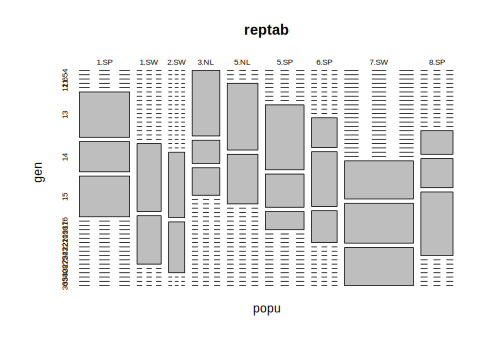
\includegraphics{BIO8940_book_files/figure-latex/unnamed-chunk-32-1.pdf}
\caption{\label{fig:unnamed-chunk-32}A truly useless plot no one can understand}
\end{figure}

\begin{enumerate}
\def\labelenumi{\arabic{enumi}.}
\setcounter{enumi}{1}
\tightlist
\item
  \texttt{colSums()} do the sum of all the rows for each columns of a table. So \texttt{colSums(reptab\textgreater{}0)} gives you for each genotype the number of populations (lines) where you have at least 1 observations.
\end{enumerate}

\begin{Shaded}
\begin{Highlighting}[]
\KeywordTok{colSums}\NormalTok{(reptab }\OperatorTok{>}\StringTok{ }\DecValTok{0}\NormalTok{)}
\end{Highlighting}
\end{Shaded}

\begin{verbatim}
##  4  5  6 11 12 13 14 15 16 17 18 19 20 21 22 23 24 25 27 28 30 34 35 36 
##  1  1  1  1  1  1  1  1  1  1  1  1  1  1  1  1  1  1  1  1  1  1  1  1
\end{verbatim}

\begin{Shaded}
\begin{Highlighting}[]
\KeywordTok{rowSums}\NormalTok{(reptab }\OperatorTok{>}\StringTok{ }\DecValTok{0}\NormalTok{)}
\end{Highlighting}
\end{Shaded}

\begin{verbatim}
## 1.SP 1.SW 2.SW 3.NL 5.NL 5.SP 6.SP 7.SW 8.SP 
##    3    2    2    3    2    3    3    3    3
\end{verbatim}

\begin{enumerate}
\def\labelenumi{\arabic{enumi}.}
\setcounter{enumi}{2}
\tightlist
\item
  You firts need to create a new table of number of observations per treatment and genotypes
\end{enumerate}

\begin{Shaded}
\begin{Highlighting}[]
\NormalTok{reptab2 <-}\StringTok{ }\KeywordTok{with}\NormalTok{(dat_tf, }\KeywordTok{table}\NormalTok{(}\KeywordTok{paste}\NormalTok{(amd, nutrient, }\DataTypeTok{sep =} \StringTok{"_"}\NormalTok{), gen))}
\KeywordTok{range}\NormalTok{(reptab2)}
\end{Highlighting}
\end{Shaded}

\begin{verbatim}
## [1]  2 13
\end{verbatim}

This reveals that we have only 2--4 populations per region and 2--3 genotypes per population. However, we also have 2--13 replicates per genotype for each treatment combination (four unique treatment combinations: 2 levels of nutrients by 2 levels of simulated herbivory). Thus, even though this was a reasonably large experiment (625 plants), there were a very small number of replicates with which to estimate variance components, and many more potential interactions than our data can support. Therefore, judicious selection of model terms, based on both biology and the data, is warranted. We note that we don't really have enough levels per random effect, nor enough replication per unique treatment combination. Therefore, we decide to omit the fixed effect of ``region'', although we recognize that populations in different regions are widely geographically separated.

However, as in all GLMMs where the scale parameter is treated as fixed and deviations from the fixed scale parameter would be identifiable (i.e.~Poisson and binomial (N \textgreater{} 1), but not binary, models) we may have to deal with overdispersion.

\hypertarget{look-at-overall-patterns-in-data}{%
\subsection{Look at overall patterns in data}\label{look-at-overall-patterns-in-data}}

I usually like to start with a relatively simple overall plot of the data, disregarding the random factors, just to see what's going on. For reasons to be discussed below, we choose to look at the data on the log (or log(1 + x) scale. Let's plot either box-and-whisker plots (useful summaries) or dot plots (more detailed, good for seeing if we missed anything).

\begin{figure}
\centering
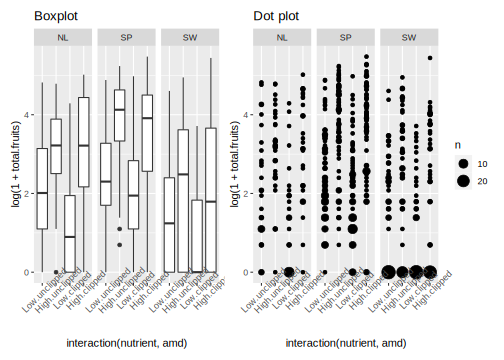
\includegraphics{BIO8940_book_files/figure-latex/unnamed-chunk-35-1.pdf}
\caption{\label{fig:unnamed-chunk-35}Number of fruits (log + 1) as a function of treatments}
\end{figure}

\begin{rmdcode}
\textbf{Exercise} generate these plots and figure out how they work before continuing. Try conditioning/faceting on population rather than region: for facet\_wrap you might want to take out the nrow=1 specification. If you want try reorder the subplots by overall mean fruit set and/or colour the points according to the region they come from.
\end{rmdcode}

\begin{Shaded}
\begin{Highlighting}[]
\NormalTok{p1 <-}\StringTok{ }\KeywordTok{qplot}\NormalTok{(}
    \KeywordTok{interaction}\NormalTok{(nutrient, amd),}
    \KeywordTok{log}\NormalTok{(}\DecValTok{1} \OperatorTok{+}\StringTok{ }\NormalTok{total.fruits),}
    \DataTypeTok{data =}\NormalTok{ dat_tf, }\DataTypeTok{geom =} \StringTok{"boxplot"}\NormalTok{) }\OperatorTok{+}
\StringTok{  }\KeywordTok{facet_wrap}\NormalTok{(}\OperatorTok{~}\NormalTok{reg, }\DataTypeTok{nrow =} \DecValTok{1}\NormalTok{) }\OperatorTok{+}
\StringTok{  }\KeywordTok{theme}\NormalTok{(}\DataTypeTok{axis.text.x =} \KeywordTok{element_text}\NormalTok{(}\DataTypeTok{angle =} \DecValTok{45}\NormalTok{)) }\OperatorTok{+}
\StringTok{  }\KeywordTok{ggtitle}\NormalTok{(}\StringTok{"Boxplot"}\NormalTok{)}
\NormalTok{p2 <-}\StringTok{ }\KeywordTok{qplot}\NormalTok{(}
    \KeywordTok{interaction}\NormalTok{(nutrient, amd),}
    \KeywordTok{log}\NormalTok{(}\DecValTok{1} \OperatorTok{+}\StringTok{ }\NormalTok{total.fruits),}
    \DataTypeTok{data =}\NormalTok{ dat_tf) }\OperatorTok{+}
\StringTok{  }\KeywordTok{facet_wrap}\NormalTok{(}\OperatorTok{~}\NormalTok{reg, }\DataTypeTok{nrow =} \DecValTok{1}\NormalTok{) }\OperatorTok{+}
\StringTok{  }\KeywordTok{stat_sum}\NormalTok{() }\OperatorTok{+}
\StringTok{  }\KeywordTok{theme}\NormalTok{(}\DataTypeTok{axis.text.x =} \KeywordTok{element_text}\NormalTok{(}\DataTypeTok{angle =} \DecValTok{45}\NormalTok{)) }\OperatorTok{+}
\StringTok{  }\KeywordTok{ggtitle}\NormalTok{(}\StringTok{"Dot plot"}\NormalTok{)}
\NormalTok{p1 }\OperatorTok{+}\StringTok{ }\NormalTok{p2}
\end{Highlighting}
\end{Shaded}

\hypertarget{choose-an-error-distribution}{%
\subsection{Choose an error distribution}\label{choose-an-error-distribution}}

The data are non-normal in principle (i.e., count data, so our first guess would be a Poisson distribution). If we transform total fruits with the canonical link function (log), we hope to see relatively homogeneous variances across categories and groups.

First we define a new factor that represents every combination of genotype and treatment (nutrient × clipping) treatment, and sort it in order of increasing mean fruit set.

\begin{Shaded}
\begin{Highlighting}[]
\NormalTok{dat_tf <-}\StringTok{ }\NormalTok{dat_tf }\OperatorTok
\StringTok{  }\KeywordTok{mutate}\NormalTok{(}
    \DataTypeTok{gna =} \KeywordTok{interaction}\NormalTok{(gen, nutrient, amd),}
    \DataTypeTok{gna =} \KeywordTok{fct_reorder}\NormalTok{(gna, total.fruits, mean)}
\NormalTok{  )}
\end{Highlighting}
\end{Shaded}

Now time to plot it

\begin{Shaded}
\begin{Highlighting}[]
\KeywordTok{ggplot}\NormalTok{(dat_tf, }\KeywordTok{aes}\NormalTok{(}\DataTypeTok{x =}\NormalTok{ gna, }\DataTypeTok{y =} \KeywordTok{log}\NormalTok{(}\DecValTok{1} \OperatorTok{+}\StringTok{ }\NormalTok{total.fruits))) }\OperatorTok{+}
\StringTok{  }\KeywordTok{geom_boxplot}\NormalTok{() }\OperatorTok{+}
\StringTok{  }\KeywordTok{theme_bw}\NormalTok{() }\OperatorTok{+}
\StringTok{  }\KeywordTok{theme}\NormalTok{(}\DataTypeTok{axis.text.x =} \KeywordTok{element_text}\NormalTok{(}\DataTypeTok{angle =} \DecValTok{90}\NormalTok{))}
\end{Highlighting}
\end{Shaded}

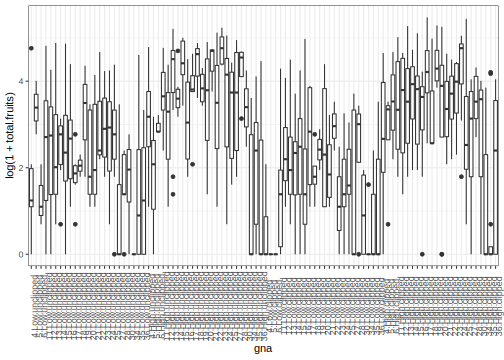
\includegraphics{BIO8940_book_files/figure-latex/unnamed-chunk-39-1.pdf}

We could also calculate the variance for each genotype × treatment combination and provide a statistical summary of these variances.
This reveals substantial variation among the sample variances on the transformed data. In addition to heterogeneous variances across groups, Figure 1 reveals many zeroes in groups, and some groups with a mean and variance of zero, further suggesting we need a non-normal error distribution, and perhaps something other than a Poisson distribution.

We could calculate λ(mean) for each genotype × treatment combination and provide a statistical summary of each group's λ.

\begin{Shaded}
\begin{Highlighting}[]
\NormalTok{grp_means <-}\StringTok{ }\KeywordTok{with}\NormalTok{(dat_tf, }\KeywordTok{tapply}\NormalTok{(total.fruits, }\KeywordTok{list}\NormalTok{(gna), mean))}
\KeywordTok{summary}\NormalTok{(grp_means)}
\end{Highlighting}
\end{Shaded}

\begin{verbatim}
##    Min. 1st Qu.  Median    Mean 3rd Qu.    Max. 
##    0.00   11.35   23.16   31.86   49.74  122.40
\end{verbatim}

A core property of the Poisson distribution is that the variance is equal to the mean. A simple diagnostic is a plot of the group variances against the group means:

\begin{itemize}
\tightlist
\item
  Poisson-distributed data will result in a linear pattern with slope = 1
\item
  as long as the variance is generally greater than the mean, we call the data overdispersed. Overdispersion comes in various forms:

  \begin{itemize}
  \tightlist
  \item
    a linear mean-variance relationship with Var = φµ (a line through the origin) with φ \textgreater{} 1 is called a quasi-Poisson pattern (this term describes the mean-variance relationship, not any particular proability distribution); we can implement it statistically via quasilikelihood (Venables and Ripley, 2002) or by using a particular parameterization of the negative binomial distribution (``NB1'' inthe terminology of Hardin and Hilbe (2007))
  \item
    a semi-quadratic pattern, Var = µ(1 + αµ) or µ(1 + µ/k), is characteristic of overdispersed data that is driven by underlying heterogeneity among samples, either the negative binomial (gamma-Poisson) or the lognormal-Poisson \citep{elston2001}
  \end{itemize}
\end{itemize}

We've already calculated the group (genotype × treatment) means, we calculate the variances in the same way.

\begin{Shaded}
\begin{Highlighting}[]
\NormalTok{grp_vars <-}\StringTok{ }\KeywordTok{with}\NormalTok{(}
\NormalTok{  dat_tf,}
  \KeywordTok{tapply}\NormalTok{(}
\NormalTok{    total.fruits,}
    \KeywordTok{list}\NormalTok{(gna), var}
\NormalTok{  )}
\NormalTok{)}
\end{Highlighting}
\end{Shaded}

We can get approximate estimates of the quasi-Poisson (linear) and negative binomial (linear/quadratic) pattern using lm.

\begin{Shaded}
\begin{Highlighting}[]
\NormalTok{lm1 <-}\StringTok{ }\KeywordTok{lm}\NormalTok{(grp_vars }\OperatorTok{~}\StringTok{ }\NormalTok{grp_means }\OperatorTok{-}\StringTok{ }\DecValTok{1}\NormalTok{) }\CommentTok{## `quasi-Poisson' fit}
\NormalTok{phi_fit <-}\StringTok{ }\KeywordTok{coef}\NormalTok{(lm1)}
\NormalTok{lm2 <-}\StringTok{ }\KeywordTok{lm}\NormalTok{((grp_vars }\OperatorTok{-}\StringTok{ }\NormalTok{grp_means) }\OperatorTok{~}\StringTok{ }\KeywordTok{I}\NormalTok{(grp_means}\OperatorTok{^}\DecValTok{2}\NormalTok{) }\OperatorTok{-}\StringTok{ }\DecValTok{1}\NormalTok{)}
\NormalTok{k_fit <-}\StringTok{ }\DecValTok{1} \OperatorTok{/}\StringTok{ }\KeywordTok{coef}\NormalTok{(lm2)}
\end{Highlighting}
\end{Shaded}

Now we can plot them.

\begin{Shaded}
\begin{Highlighting}[]
\KeywordTok{plot}\NormalTok{(grp_vars }\OperatorTok{~}\StringTok{ }\NormalTok{grp_means, }\DataTypeTok{xlab =} \StringTok{"group means"}\NormalTok{, }\DataTypeTok{ylab =} \StringTok{"group variances"}\NormalTok{)}
\KeywordTok{abline}\NormalTok{(}\KeywordTok{c}\NormalTok{(}\DecValTok{0}\NormalTok{, }\DecValTok{1}\NormalTok{), }\DataTypeTok{lty =} \DecValTok{2}\NormalTok{)}
\KeywordTok{text}\NormalTok{(}\DecValTok{105}\NormalTok{, }\DecValTok{500}\NormalTok{, }\StringTok{"Poisson"}\NormalTok{)}
\KeywordTok{curve}\NormalTok{(phi_fit }\OperatorTok{*}\StringTok{ }\NormalTok{x, }\DataTypeTok{col =} \DecValTok{2}\NormalTok{, }\DataTypeTok{add =} \OtherTok{TRUE}\NormalTok{)}
\CommentTok{## bquote() is used to substitute numeric values}
\CommentTok{## in equations with symbols}
\KeywordTok{text}\NormalTok{(}\DecValTok{110}\NormalTok{, }\DecValTok{3900}\NormalTok{,}
  \KeywordTok{bquote}\NormalTok{(}\KeywordTok{paste}\NormalTok{(}\StringTok{"QP: "}\NormalTok{, sigma}\OperatorTok{^}\DecValTok{2} \OperatorTok{==}\StringTok{ }\NormalTok{.(}\KeywordTok{round}\NormalTok{(phi_fit, }\DecValTok{1}\NormalTok{)) }\OperatorTok{*}\StringTok{ }\NormalTok{mu)),}
  \DataTypeTok{col =} \DecValTok{2}
\NormalTok{)}
\KeywordTok{curve}\NormalTok{(x }\OperatorTok{*}\StringTok{ }\NormalTok{(}\DecValTok{1} \OperatorTok{+}\StringTok{ }\NormalTok{x }\OperatorTok{/}\StringTok{ }\NormalTok{k_fit), }\DataTypeTok{col =} \DecValTok{4}\NormalTok{, }\DataTypeTok{add =} \OtherTok{TRUE}\NormalTok{)}
\KeywordTok{text}\NormalTok{(}\DecValTok{104}\NormalTok{, }\DecValTok{7200}\NormalTok{, }\KeywordTok{paste}\NormalTok{(}\StringTok{"NB: k="}\NormalTok{, }\KeywordTok{round}\NormalTok{(k_fit, }\DecValTok{1}\NormalTok{), }\DataTypeTok{sep =} \StringTok{""}\NormalTok{), }\DataTypeTok{col =} \DecValTok{4}\NormalTok{)}
\NormalTok{l_fit <-}\StringTok{ }\KeywordTok{loess}\NormalTok{(grp_vars }\OperatorTok{~}\StringTok{ }\NormalTok{grp_means)}
\NormalTok{mvec <-}\StringTok{ }\DecValTok{0}\OperatorTok{:}\DecValTok{120}
\KeywordTok{lines}\NormalTok{(mvec, }\KeywordTok{predict}\NormalTok{(l_fit, mvec), }\DataTypeTok{col =} \DecValTok{5}\NormalTok{)}
\KeywordTok{text}\NormalTok{(}\DecValTok{100}\NormalTok{, }\DecValTok{2500}\NormalTok{, }\StringTok{"loess"}\NormalTok{, }\DataTypeTok{col =} \DecValTok{5}\NormalTok{)}
\end{Highlighting}
\end{Shaded}

\begin{figure}
\centering
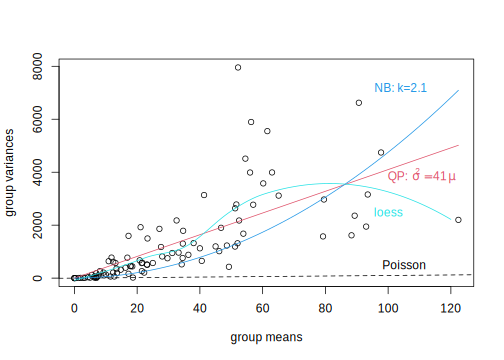
\includegraphics{BIO8940_book_files/figure-latex/unnamed-chunk-43-1.pdf}
\caption{\label{fig:unnamed-chunk-43}Graphical evaluation of distribution to use}
\end{figure}

Same with ggplot

\begin{Shaded}
\begin{Highlighting}[]
\KeywordTok{ggplot}\NormalTok{(}
  \KeywordTok{data.frame}\NormalTok{(grp_means, grp_vars),}
  \KeywordTok{aes}\NormalTok{(}\DataTypeTok{x =}\NormalTok{ grp_means, }\DataTypeTok{y =}\NormalTok{ grp_vars)) }\OperatorTok{+}
\StringTok{  }\KeywordTok{geom_point}\NormalTok{() }\OperatorTok{+}
\StringTok{  }\KeywordTok{geom_smooth}\NormalTok{(}
    \KeywordTok{aes}\NormalTok{(}\DataTypeTok{colour =} \StringTok{"Loess"}\NormalTok{), }\DataTypeTok{se =} \OtherTok{FALSE}\NormalTok{) }\OperatorTok{+}
\StringTok{  }\KeywordTok{geom_smooth}\NormalTok{(}
    \DataTypeTok{method =} \StringTok{"lm"}\NormalTok{, }\DataTypeTok{formula =}\NormalTok{ y }\OperatorTok{~}\StringTok{ }\NormalTok{x }\OperatorTok{-}\StringTok{ }\DecValTok{1}\NormalTok{, }\DataTypeTok{se =} \OtherTok{FALSE}\NormalTok{,}
    \KeywordTok{aes}\NormalTok{(}\DataTypeTok{colour =} \StringTok{"Q_Pois"}\NormalTok{)) }\OperatorTok{+}
\StringTok{  }\KeywordTok{stat_function}\NormalTok{(}
    \DataTypeTok{fun =} \ControlFlowTok{function}\NormalTok{(x) x }\OperatorTok{*}\StringTok{ }\NormalTok{(}\DecValTok{1} \OperatorTok{+}\StringTok{ }\NormalTok{x }\OperatorTok{/}\StringTok{ }\NormalTok{k_fit),}
    \KeywordTok{aes}\NormalTok{(}\DataTypeTok{colour =} \StringTok{"Neg_bin"}\NormalTok{)}
\NormalTok{  ) }\OperatorTok{+}
\StringTok{  }\KeywordTok{geom_abline}\NormalTok{(}
    \KeywordTok{aes}\NormalTok{(}\DataTypeTok{intercept =} \DecValTok{0}\NormalTok{, }\DataTypeTok{slope =} \DecValTok{1}\NormalTok{, }\DataTypeTok{colour =} \StringTok{"Poisson"}\NormalTok{)) }\OperatorTok{+}
\StringTok{  }\KeywordTok{scale_colour_manual}\NormalTok{(}
    \DataTypeTok{name =} \StringTok{"legend"}\NormalTok{,}
    \DataTypeTok{values =} \KeywordTok{c}\NormalTok{(}\StringTok{"blue"}\NormalTok{, }\StringTok{"purple"}\NormalTok{, }\StringTok{"black"}\NormalTok{, }\StringTok{"red"}\NormalTok{)) }\OperatorTok{+}
\StringTok{  }\KeywordTok{scale_fill_manual}\NormalTok{(}
    \DataTypeTok{name =} \StringTok{"legend"}\NormalTok{,}
    \DataTypeTok{values =} \KeywordTok{c}\NormalTok{(}\StringTok{"blue"}\NormalTok{, }\StringTok{"purple"}\NormalTok{, }\StringTok{"black"}\NormalTok{, }\StringTok{"red"}\NormalTok{)) }\OperatorTok{+}
\StringTok{  }\KeywordTok{guides}\NormalTok{(}\DataTypeTok{fill =} \OtherTok{FALSE}\NormalTok{)}
\end{Highlighting}
\end{Shaded}

\begin{verbatim}
## `geom_smooth()` using method = 'loess' and formula 'y ~ x'
\end{verbatim}

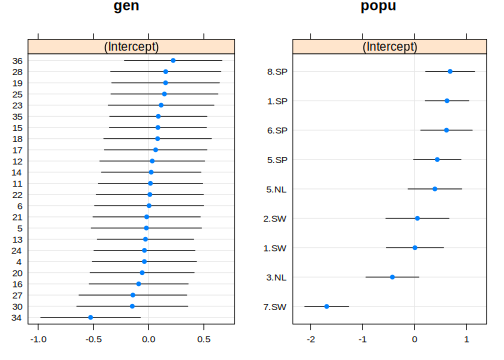
\includegraphics{BIO8940_book_files/figure-latex/unnamed-chunk-44-1.pdf}

These fits are not rigorous statistical tests --- they violate a variety of assumptions of linear regression (e.g.~constant variance, independence), but they are good enough to give us an initial guess about what distributions we should use.

\textbf{Exercise}

\begin{itemize}
\tightlist
\item
  compare a simple quadratic fit to the data (i.e., without the linear part) with the negative binomial and quasipoisson fits
\end{itemize}

\begin{Shaded}
\begin{Highlighting}[]
\NormalTok{lm3 <-}\StringTok{ }\KeywordTok{lm}\NormalTok{(grp_vars }\OperatorTok{~}\StringTok{ }\KeywordTok{I}\NormalTok{(grp_means)}\OperatorTok{^}\DecValTok{2} \OperatorTok{-}\StringTok{ }\DecValTok{1}\NormalTok{) }\CommentTok{## quadratic fit}
\NormalTok{quad_fit <-}\StringTok{ }\KeywordTok{coef}\NormalTok{(lm3)}

\KeywordTok{ggplot}\NormalTok{(}
  \KeywordTok{data.frame}\NormalTok{(grp_means, grp_vars),}
  \KeywordTok{aes}\NormalTok{(}\DataTypeTok{x =}\NormalTok{ grp_means, }\DataTypeTok{y =}\NormalTok{ grp_vars)) }\OperatorTok{+}
\StringTok{  }\KeywordTok{geom_point}\NormalTok{() }\OperatorTok{+}
\StringTok{  }\KeywordTok{geom_smooth}\NormalTok{(}
    \DataTypeTok{method =} \StringTok{"lm"}\NormalTok{, }\DataTypeTok{formula =}\NormalTok{ y }\OperatorTok{~}\StringTok{ }\NormalTok{x }\OperatorTok{-}\StringTok{ }\DecValTok{1}\NormalTok{, }\DataTypeTok{se =} \OtherTok{FALSE}\NormalTok{,}
    \KeywordTok{aes}\NormalTok{(}\DataTypeTok{colour =} \StringTok{"Q_Pois"}\NormalTok{)) }\OperatorTok{+}
\StringTok{  }\KeywordTok{stat_function}\NormalTok{(}
    \DataTypeTok{fun =} \ControlFlowTok{function}\NormalTok{(x) x }\OperatorTok{*}\StringTok{ }\NormalTok{(}\DecValTok{1} \OperatorTok{+}\StringTok{ }\NormalTok{x }\OperatorTok{/}\StringTok{ }\NormalTok{k_fit),}
    \KeywordTok{aes}\NormalTok{(}\DataTypeTok{colour =} \StringTok{"Neg_bin"}\NormalTok{)}
\NormalTok{  ) }\OperatorTok{+}
\StringTok{  }\KeywordTok{geom_smooth}\NormalTok{(}
    \DataTypeTok{method =} \StringTok{"lm"}\NormalTok{, }\DataTypeTok{formula =}\NormalTok{ y }\OperatorTok{~}\StringTok{ }\KeywordTok{I}\NormalTok{(x}\OperatorTok{^}\DecValTok{2}\NormalTok{) }\OperatorTok{-}\StringTok{ }\DecValTok{1}\NormalTok{, }\DataTypeTok{se =} \OtherTok{FALSE}\NormalTok{,}
    \KeywordTok{aes}\NormalTok{(}\DataTypeTok{colour =} \StringTok{"Quad"}\NormalTok{)) }\OperatorTok{+}
\StringTok{  }\KeywordTok{scale_colour_manual}\NormalTok{(}
    \DataTypeTok{name =} \StringTok{"legend"}\NormalTok{,}
    \DataTypeTok{values =} \KeywordTok{c}\NormalTok{(}\StringTok{"blue"}\NormalTok{, }\StringTok{"purple"}\NormalTok{, }\StringTok{"black"}\NormalTok{)) }\OperatorTok{+}
\StringTok{  }\KeywordTok{scale_fill_manual}\NormalTok{(}
    \DataTypeTok{name =} \StringTok{"legend"}\NormalTok{,}
    \DataTypeTok{values =} \KeywordTok{c}\NormalTok{(}\StringTok{"blue"}\NormalTok{, }\StringTok{"purple"}\NormalTok{, }\StringTok{"black"}\NormalTok{)) }\OperatorTok{+}
\StringTok{  }\KeywordTok{guides}\NormalTok{(}\DataTypeTok{fill =} \OtherTok{FALSE}\NormalTok{)}
\end{Highlighting}
\end{Shaded}

\begin{figure}
\centering
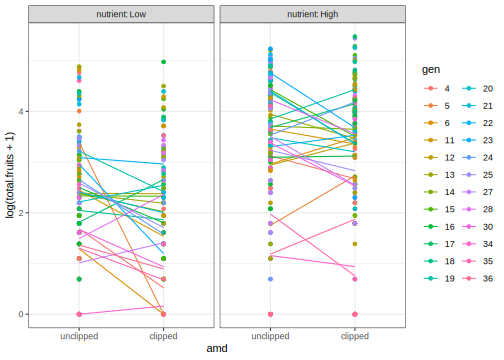
\includegraphics{BIO8940_book_files/figure-latex/unnamed-chunk-45-1.pdf}
\caption{\label{fig:unnamed-chunk-45}Graphical evaluation of distribution to use including quadratic effect}
\end{figure}

\hypertarget{plotting-the-response-vs-treatments}{%
\subsubsection{Plotting the response vs treatments}\label{plotting-the-response-vs-treatments}}

Just to avoid surprises

\begin{Shaded}
\begin{Highlighting}[]
\KeywordTok{ggplot}\NormalTok{(dat_tf, }\KeywordTok{aes}\NormalTok{(}\DataTypeTok{x =}\NormalTok{ amd, }\DataTypeTok{y =} \KeywordTok{log}\NormalTok{(total.fruits }\OperatorTok{+}\StringTok{ }\DecValTok{1}\NormalTok{), }\DataTypeTok{colour =}\NormalTok{ nutrient)) }\OperatorTok{+}
\StringTok{  }\KeywordTok{geom_point}\NormalTok{() }\OperatorTok{+}
\StringTok{  }\CommentTok{## need to use as.numeric(amd) to get lines}
\StringTok{  }\KeywordTok{stat_summary}\NormalTok{(}\KeywordTok{aes}\NormalTok{(}\DataTypeTok{x =} \KeywordTok{as.numeric}\NormalTok{(amd)), }\DataTypeTok{fun =}\NormalTok{ mean, }\DataTypeTok{geom =} \StringTok{"line"}\NormalTok{) }\OperatorTok{+}
\StringTok{  }\KeywordTok{theme_bw}\NormalTok{() }\OperatorTok{+}
\StringTok{  }\KeywordTok{theme}\NormalTok{(}\DataTypeTok{panel.spacing =} \KeywordTok{unit}\NormalTok{(}\DecValTok{0}\NormalTok{, }\StringTok{"lines"}\NormalTok{)) }\OperatorTok{+}
\StringTok{  }\KeywordTok{facet_wrap}\NormalTok{(}\OperatorTok{~}\NormalTok{popu)}
\end{Highlighting}
\end{Shaded}

\begin{figure}
\centering
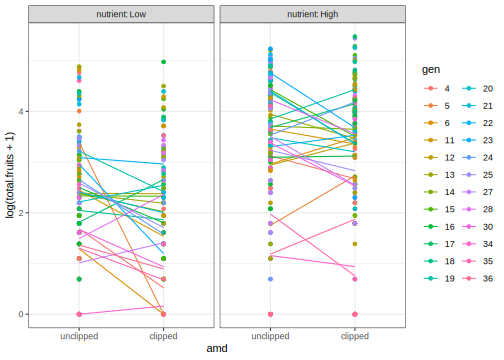
\includegraphics{BIO8940_book_files/figure-latex/unnamed-chunk-46-1.pdf}
\caption{\label{fig:unnamed-chunk-46}Fruit production by treatments by population}
\end{figure}

\begin{Shaded}
\begin{Highlighting}[]
\KeywordTok{ggplot}\NormalTok{(dat_tf, }\KeywordTok{aes}\NormalTok{(}\DataTypeTok{x =}\NormalTok{ amd, }\DataTypeTok{y =} \KeywordTok{log}\NormalTok{(total.fruits }\OperatorTok{+}\StringTok{ }\DecValTok{1}\NormalTok{), }\DataTypeTok{colour =}\NormalTok{ gen)) }\OperatorTok{+}
\StringTok{  }\KeywordTok{geom_point}\NormalTok{() }\OperatorTok{+}
\StringTok{  }\KeywordTok{stat_summary}\NormalTok{(}\KeywordTok{aes}\NormalTok{(}\DataTypeTok{x =} \KeywordTok{as.numeric}\NormalTok{(amd)), }\DataTypeTok{fun =}\NormalTok{ mean, }\DataTypeTok{geom =} \StringTok{"line"}\NormalTok{) }\OperatorTok{+}
\StringTok{  }\KeywordTok{theme_bw}\NormalTok{() }\OperatorTok{+}
\StringTok{  }\CommentTok{## label_both adds variable name ('nutrient') to facet labels}
\StringTok{  }\KeywordTok{facet_grid}\NormalTok{(. }\OperatorTok{~}\StringTok{ }\NormalTok{nutrient, }\DataTypeTok{labeller =}\NormalTok{ label_both)}
\end{Highlighting}
\end{Shaded}

\begin{figure}
\centering
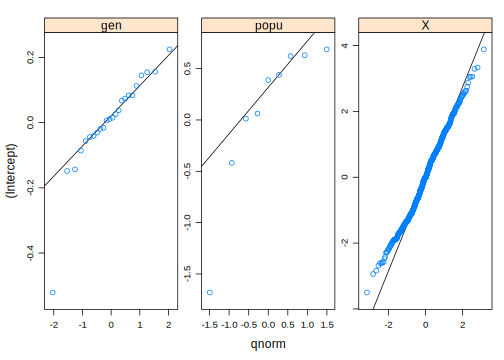
\includegraphics{BIO8940_book_files/figure-latex/unnamed-chunk-47-1.pdf}
\caption{\label{fig:unnamed-chunk-47}Fruit production by genotype by treatments}
\end{figure}

\hypertarget{fitting-group-wise-glm}{%
\subsection{Fitting group-wise GLM}\label{fitting-group-wise-glm}}

Another general starting approach is to fit GLMs to each group of data separately, equivalent to treating the grouping variables as fixed effects.
This should result in reasonable variation among treatment effects. We first fit the models, and then examine the coefficients.

\begin{Shaded}
\begin{Highlighting}[]
\NormalTok{glm_lis <-}\StringTok{ }\KeywordTok{lmList}\NormalTok{(}
\NormalTok{  total.fruits }\OperatorTok{~}\StringTok{ }\NormalTok{nutrient }\OperatorTok{*}\StringTok{ }\NormalTok{amd }\OperatorTok{|}\StringTok{ }\NormalTok{gen,}
  \DataTypeTok{data =}\NormalTok{ dat_tf,}
  \DataTypeTok{family =} \StringTok{"poisson"}\NormalTok{)}
\KeywordTok{plot.lmList}\NormalTok{(glm_lis)}
\end{Highlighting}
\end{Shaded}

\begin{verbatim}
## Using grp as id variables
\end{verbatim}

\begin{figure}
\centering
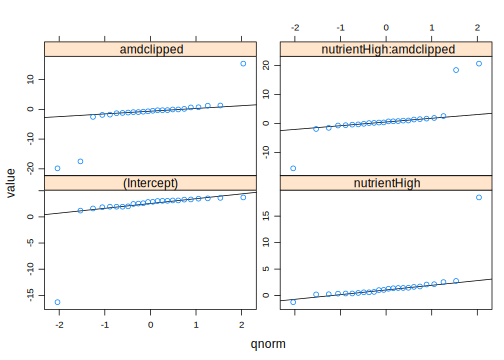
\includegraphics{BIO8940_book_files/figure-latex/unnamed-chunk-48-1.pdf}
\caption{\label{fig:unnamed-chunk-48}Model coefficients for GLM fits on each genotype}
\end{figure}

Three genotypes (5, 6, 34) have extreme coefficients (Fig. 5). A mixed model assumes that the underlying random effects are normally distributed, although we shouldn't take these outliers too seriously at this point --- we are not actually plotting the random effects, or even estimates of random effects (which are not themselves guaranteed to be normally distributed), but rather separate estimates for each group.
Create a plotting function for Q-Q plots of these coefficients to visualize the departure from normality.

\begin{Shaded}
\begin{Highlighting}[]
\KeywordTok{qqmath.lmList}\NormalTok{(glm_lis)}
\end{Highlighting}
\end{Shaded}

\begin{verbatim}
## Using  as id variables
\end{verbatim}

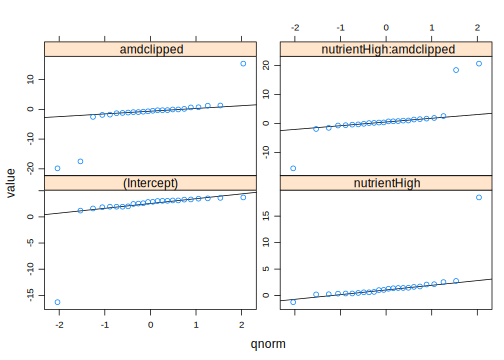
\includegraphics{BIO8940_book_files/figure-latex/unnamed-chunk-49-1.pdf}
We see that these extreme coefficients fall far outside a normal error distribution. We shouldn't take these outliers too seriously at this point --- we are not actually plotting the random effects, or even estimates of random effects, but rather separate estimates for each group.
Especially if these groups have relatively small sample sizes, the estimates may eventually be ``shrunk'' closer to the mean when we do the mixed model.
We should nonetheless take care to see if the coefficients for these genotypes from the GLMM are still outliers, and take the same precautions as we usually do for outliers. For example, we can look back at the original data to see if there is something weird about the way those genotypes were collected, or try re-running the analysis without those genotypes to see if the results are robust.

\hypertarget{fitting-and-evaluating-glmms}{%
\subsection{Fitting and evaluating GLMMs}\label{fitting-and-evaluating-glmms}}

Now we (try to) build and fit a full model, using \texttt{glmer} in the \texttt{emo::ji("pacakage")} \texttt{lme4}. This model has random effects for all genotype and population × treatment random effects, and for the nuisance variables for the rack and germination method (status). (Given the mean-variance relationship we saw it's pretty clear that we are going to have to proceed eventually to a model with overdispersion, but we fit the Poisson model first for illustration.)

\begin{Shaded}
\begin{Highlighting}[]
\NormalTok{mp1 <-}\StringTok{ }\KeywordTok{glmer}\NormalTok{(total.fruits }\OperatorTok{~}\StringTok{ }\NormalTok{nutrient }\OperatorTok{*}\StringTok{ }\NormalTok{amd }\OperatorTok{+}
\StringTok{  }\NormalTok{rack }\OperatorTok{+}\StringTok{ }\NormalTok{status }\OperatorTok{+}
\StringTok{  }\NormalTok{(amd }\OperatorTok{*}\StringTok{ }\NormalTok{nutrient }\OperatorTok{|}\StringTok{ }\NormalTok{popu) }\OperatorTok{+}
\StringTok{  }\NormalTok{(amd }\OperatorTok{*}\StringTok{ }\NormalTok{nutrient }\OperatorTok{|}\StringTok{ }\NormalTok{gen),}
\DataTypeTok{data =}\NormalTok{ dat_tf, }\DataTypeTok{family =} \StringTok{"poisson"}
\NormalTok{)}
\end{Highlighting}
\end{Shaded}

\begin{verbatim}
## Warning in checkConv(attr(opt, "derivs"), opt$par, ctrl = control$checkConv, :
## Model failed to converge with max|grad| = 0.0132432 (tol = 0.002, component 1)
\end{verbatim}

\begin{Shaded}
\begin{Highlighting}[]
\KeywordTok{overdisp_fun}\NormalTok{(mp1)}
\end{Highlighting}
\end{Shaded}

\begin{verbatim}
##       chisq       ratio           p 
## 13909.46562    23.25998     0.00000
\end{verbatim}

We can ignore the model convergence for the moment. This shows that the data are (extremely) over-dispersed, given the model.

Now we add the observation-level random effect to the model to account for overdispersion \citep{elston2001}.

\begin{Shaded}
\begin{Highlighting}[]
\NormalTok{mp2 <-}\StringTok{ }\KeywordTok{update}\NormalTok{(mp1, . }\OperatorTok{~}\StringTok{ }\NormalTok{. }\OperatorTok{+}\StringTok{ }\NormalTok{(}\DecValTok{1} \OperatorTok{|}\StringTok{ }\NormalTok{X))}
\end{Highlighting}
\end{Shaded}

\begin{verbatim}
## Warning in (function (fn, par, lower = rep.int(-Inf, n), upper = rep.int(Inf, :
## failure to converge in 10000 evaluations
\end{verbatim}

\begin{verbatim}
## Warning in optwrap(optimizer, devfun, start, rho$lower, control = control, :
## convergence code 4 from Nelder_Mead: failure to converge in 10000 evaluations
\end{verbatim}

\begin{verbatim}
## Warning in checkConv(attr(opt, "derivs"), opt$par, ctrl = control$checkConv, :
## Model failed to converge with max|grad| = 0.169728 (tol = 0.002, component 1)
\end{verbatim}

The model takes much longer to fit (and gives warnings).
We look just at the variance components. In particular, if we look at the correlation matrix among the genotype random effects, we see a perfect
correlation.

\begin{Shaded}
\begin{Highlighting}[]
\KeywordTok{attr}\NormalTok{(}\KeywordTok{VarCorr}\NormalTok{(mp2)}\OperatorTok{$}\NormalTok{gen, }\StringTok{"correlation"}\NormalTok{)}
\end{Highlighting}
\end{Shaded}

\begin{verbatim}
##                         (Intercept) amdclipped nutrientHigh
## (Intercept)               1.0000000 -0.9991408   -0.9877061
## amdclipped               -0.9991408  1.0000000    0.9916060
## nutrientHigh             -0.9877061  0.9916060    1.0000000
## amdclipped:nutrientHigh   0.8225706 -0.8397183   -0.9012402
##                         amdclipped:nutrientHigh
## (Intercept)                           0.8225706
## amdclipped                           -0.8397183
## nutrientHigh                         -0.9012402
## amdclipped:nutrientHigh               1.0000000
\end{verbatim}

We'll try getting rid of the correlations between clipping (\texttt{amd}) and nutrients, using \texttt{amd+nutrient} instead of \texttt{amd*nutrient} in the random effects specification (here it seems easier to re-do the model rather than using update to add and subtract terms).

\begin{Shaded}
\begin{Highlighting}[]
\NormalTok{mp3 <-}\StringTok{ }\KeywordTok{glmer}\NormalTok{(total.fruits }\OperatorTok{~}\StringTok{ }\NormalTok{nutrient }\OperatorTok{*}\StringTok{ }\NormalTok{amd }\OperatorTok{+}
\StringTok{  }\NormalTok{rack }\OperatorTok{+}\StringTok{ }\NormalTok{status }\OperatorTok{+}
\StringTok{  }\NormalTok{(amd }\OperatorTok{+}\StringTok{ }\NormalTok{nutrient }\OperatorTok{|}\StringTok{ }\NormalTok{popu) }\OperatorTok{+}
\StringTok{  }\NormalTok{(amd }\OperatorTok{+}\StringTok{ }\NormalTok{nutrient }\OperatorTok{|}\StringTok{ }\NormalTok{gen) }\OperatorTok{+}\StringTok{ }\NormalTok{(}\DecValTok{1} \OperatorTok{|}\StringTok{ }\NormalTok{X),}
\DataTypeTok{data =}\NormalTok{ dat_tf, }\DataTypeTok{family =} \StringTok{"poisson"}
\NormalTok{)}
\end{Highlighting}
\end{Shaded}

\begin{verbatim}
## Warning in checkConv(attr(opt, "derivs"), opt$par, ctrl = control$checkConv, :
## Model failed to converge with max|grad| = 0.17819 (tol = 0.002, component 1)
\end{verbatim}

\begin{Shaded}
\begin{Highlighting}[]
\KeywordTok{attr}\NormalTok{(}\KeywordTok{VarCorr}\NormalTok{(mp3)}\OperatorTok{$}\NormalTok{gen, }\StringTok{"correlation"}\NormalTok{)}
\end{Highlighting}
\end{Shaded}

\begin{verbatim}
##              (Intercept) amdclipped nutrientHigh
## (Intercept)    1.0000000 -0.7762341   -0.9979863
## amdclipped    -0.7762341  1.0000000    0.7743002
## nutrientHigh  -0.9979863  0.7743002    1.0000000
\end{verbatim}

\begin{Shaded}
\begin{Highlighting}[]
\KeywordTok{attr}\NormalTok{(}\KeywordTok{VarCorr}\NormalTok{(mp3)}\OperatorTok{$}\NormalTok{popu, }\StringTok{"correlation"}\NormalTok{)}
\end{Highlighting}
\end{Shaded}

\begin{verbatim}
##              (Intercept) amdclipped nutrientHigh
## (Intercept)    1.0000000  0.9995678    0.9973568
## amdclipped     0.9995678  1.0000000    0.9961872
## nutrientHigh   0.9973568  0.9961872    1.0000000
\end{verbatim}

Unfortunately, we still have perfect correlations among the random effects terms. For some models (e.g.~random-slope models), it is possible to fit random effects models in such a way that the correlation between the different parameters (intercept and slope in the case of random-slope models) is constrained to be zero, by fitting a model like \texttt{(1\textbar{}f)+(0+x\textbar{}f)}; unfortunately, because of the way lme4 is set up, this is considerably more difficult with categorical predictors (factors).

We have to reduce the model further in some way in order not to overfit (i.e., in order to not have perfect ±1 correlations among random effects). It looks like we can't allow both nutrients and clipping in the random effect model at either the population or the genotype level. However, it's hard to know whether we should proceed with amd or nutrient, both, or neither in the model.

A convenient way to proceed if we are going to try fitting several different combinations of random effects is to fit the model with all the fixed effects but only observation-level random effects, and then to use update to add various components to it.

\begin{Shaded}
\begin{Highlighting}[]
\NormalTok{mp_obs <-}\StringTok{ }\KeywordTok{glmer}\NormalTok{(total.fruits }\OperatorTok{~}\StringTok{ }\NormalTok{nutrient }\OperatorTok{*}\StringTok{ }\NormalTok{amd }\OperatorTok{+}
\StringTok{  }\NormalTok{rack }\OperatorTok{+}\StringTok{ }\NormalTok{status }\OperatorTok{+}
\StringTok{  }\NormalTok{(}\DecValTok{1} \OperatorTok{|}\StringTok{ }\NormalTok{X),}
\DataTypeTok{data =}\NormalTok{ dat_tf, }\DataTypeTok{family =} \StringTok{"poisson"}
\NormalTok{)}
\end{Highlighting}
\end{Shaded}

Now, for example, \texttt{update(mp\_obs,.\textasciitilde{}.+(1\textbar{}gen)+(amd\textbar{}popu))} fits the model with intercept random effects at the genotype level and variation in clipping effects across populations.

\begin{rmdcode}
\textbf{Exercise} using update, fit the models with

\begin{enumerate}
\def\labelenumi{\arabic{enumi}.}
\tightlist
\item
  clipping variation at both genotype and population levels;
\item
  nutrient variation at both genotype and populations; convince yourself that trying to fit variation in either clipping or nutrients leads to overfitting (perfect correlations).
\item
  Fit the model with only intercept variation at the population and genotype levels, saving it as mp4; show that there is non-zero variance estimated
\end{enumerate}
\end{rmdcode}

\begin{enumerate}
\def\labelenumi{\arabic{enumi}.}
\item
\end{enumerate}

\begin{Shaded}
\begin{Highlighting}[]
\NormalTok{mpcli <-}\StringTok{ }\KeywordTok{update}\NormalTok{(mp_obs, . }\OperatorTok{~}\StringTok{ }\NormalTok{. }\OperatorTok{+}\StringTok{ }\NormalTok{(amd }\OperatorTok{|}\StringTok{ }\NormalTok{gen) }\OperatorTok{+}\StringTok{ }\NormalTok{(amd }\OperatorTok{|}\StringTok{ }\NormalTok{popu))}
\end{Highlighting}
\end{Shaded}

\begin{verbatim}
## Warning in checkConv(attr(opt, "derivs"), opt$par, ctrl = control$checkConv, :
## Model failed to converge with max|grad| = 0.118377 (tol = 0.002, component 1)
\end{verbatim}

\begin{Shaded}
\begin{Highlighting}[]
\KeywordTok{VarCorr}\NormalTok{(mpcli)}
\end{Highlighting}
\end{Shaded}

\begin{verbatim}
##  Groups Name        Std.Dev. Corr  
##  X      (Intercept) 1.431462       
##  gen    (Intercept) 0.298394       
##         amdclipped  0.045082 -0.802
##  popu   (Intercept) 0.753332       
##         amdclipped  0.130340 0.997
\end{verbatim}

\begin{enumerate}
\def\labelenumi{\arabic{enumi}.}
\setcounter{enumi}{1}
\item
\end{enumerate}

\begin{Shaded}
\begin{Highlighting}[]
\NormalTok{mpnut <-}\StringTok{ }\KeywordTok{update}\NormalTok{(mp_obs, . }\OperatorTok{~}\StringTok{ }\NormalTok{. }\OperatorTok{+}\StringTok{ }\NormalTok{(nutrient }\OperatorTok{|}\StringTok{ }\NormalTok{gen) }\OperatorTok{+}\StringTok{ }\NormalTok{(nutrient }\OperatorTok{|}\StringTok{ }\NormalTok{popu))}
\end{Highlighting}
\end{Shaded}

\begin{verbatim}
## Warning in checkConv(attr(opt, "derivs"), opt$par, ctrl = control$checkConv, :
## Model failed to converge with max|grad| = 0.0285707 (tol = 0.002, component 1)
\end{verbatim}

\begin{Shaded}
\begin{Highlighting}[]
\KeywordTok{VarCorr}\NormalTok{(mpnut)}
\end{Highlighting}
\end{Shaded}

\begin{verbatim}
##  Groups Name         Std.Dev. Corr  
##  X      (Intercept)  1.41972        
##  gen    (Intercept)  0.47822        
##         nutrientHigh 0.32578  -1.000
##  popu   (Intercept)  0.74178        
##         nutrientHigh 0.12100  1.000
\end{verbatim}

\begin{enumerate}
\def\labelenumi{\arabic{enumi}.}
\setcounter{enumi}{2}
\item
\end{enumerate}

\begin{Shaded}
\begin{Highlighting}[]
\NormalTok{mp4 <-}\StringTok{ }\KeywordTok{update}\NormalTok{(mp_obs, . }\OperatorTok{~}\StringTok{ }\NormalTok{. }\OperatorTok{+}\StringTok{ }\NormalTok{(}\DecValTok{1} \OperatorTok{|}\StringTok{ }\NormalTok{gen) }\OperatorTok{+}\StringTok{ }\NormalTok{(}\DecValTok{1} \OperatorTok{|}\StringTok{ }\NormalTok{popu))}
\end{Highlighting}
\end{Shaded}

\begin{verbatim}
## Warning in checkConv(attr(opt, "derivs"), opt$par, ctrl = control$checkConv, :
## Model failed to converge with max|grad| = 0.0256392 (tol = 0.002, component 1)
\end{verbatim}

\begin{Shaded}
\begin{Highlighting}[]
\KeywordTok{VarCorr}\NormalTok{(mp4)}
\end{Highlighting}
\end{Shaded}

\begin{verbatim}
##  Groups Name        Std.Dev.
##  X      (Intercept) 1.43206 
##  gen    (Intercept) 0.28728 
##  popu   (Intercept) 0.80614
\end{verbatim}

In other words, while it's biologically plausible that there is some variation in the nutrient or clipping effect at the genotype or population levels, with this modeling approach we really don't have enough data to speak confidently about these effects.
Let's check that mp4 no longer incorporates overdispersion (the observationlevel random effect should have taken care of it):

\begin{Shaded}
\begin{Highlighting}[]
\KeywordTok{overdisp_fun}\NormalTok{(mp4)}
\end{Highlighting}
\end{Shaded}

\begin{verbatim}
##       chisq       ratio           p 
## 177.3529154   0.2883787   1.0000000
\end{verbatim}

\hypertarget{inference}{%
\subsection{Inference}\label{inference}}

\hypertarget{random-effects}{%
\subsubsection{Random effects}\label{random-effects}}

\texttt{glmer} (\texttt{lmer}) does not return information about the standard errors or confidence intervals of the variance components.

\begin{Shaded}
\begin{Highlighting}[]
\KeywordTok{VarCorr}\NormalTok{(mp4)}
\end{Highlighting}
\end{Shaded}

\begin{verbatim}
##  Groups Name        Std.Dev.
##  X      (Intercept) 1.43206 
##  gen    (Intercept) 0.28728 
##  popu   (Intercept) 0.80614
\end{verbatim}

\hypertarget{testing-for-random-effects-1}{%
\paragraph{Testing for random Effects}\label{testing-for-random-effects-1}}

If we want to test the significance of the random effects we can fit reduced models and run likelihood ratio tests via anova, keeping in mind that in this case (testing a null hypothesis of zero variance, where the parameter is on the boundary of its feasible region) the reported p value is approximately twice what it should be.

\begin{Shaded}
\begin{Highlighting}[]
\NormalTok{mp4v1 <-}\StringTok{ }\KeywordTok{update}\NormalTok{(mp_obs, . }\OperatorTok{~}\StringTok{ }\NormalTok{. }\OperatorTok{+}\StringTok{ }\NormalTok{(}\DecValTok{1} \OperatorTok{|}\StringTok{ }\NormalTok{popu)) }\CommentTok{## popu only (drop gen)}
\NormalTok{mp4v2 <-}\StringTok{ }\KeywordTok{update}\NormalTok{(mp_obs, . }\OperatorTok{~}\StringTok{ }\NormalTok{. }\OperatorTok{+}\StringTok{ }\NormalTok{(}\DecValTok{1} \OperatorTok{|}\StringTok{ }\NormalTok{gen)) }\CommentTok{## gen only (drop popu)}
\end{Highlighting}
\end{Shaded}

\begin{verbatim}
## Warning in checkConv(attr(opt, "derivs"), opt$par, ctrl = control$checkConv, :
## unable to evaluate scaled gradient
\end{verbatim}

\begin{verbatim}
## Warning in checkConv(attr(opt, "derivs"), opt$par, ctrl = control$checkConv, :
## Model failed to converge: degenerate Hessian with 2 negative eigenvalues
\end{verbatim}

\begin{Shaded}
\begin{Highlighting}[]
\KeywordTok{anova}\NormalTok{(mp4, mp4v1)}
\end{Highlighting}
\end{Shaded}

\begin{verbatim}
## Data: dat_tf
## Models:
## mp4v1: total.fruits ~ nutrient + amd + rack + status + (1 | X) + (1 | 
## mp4v1:     popu) + nutrient:amd
## mp4: total.fruits ~ nutrient + amd + rack + status + (1 | X) + (1 | 
## mp4:     gen) + (1 | popu) + nutrient:amd
##       npar    AIC    BIC  logLik deviance  Chisq Df Pr(>Chisq)  
## mp4v1    9 5017.4 5057.4 -2499.7   4999.4                       
## mp4     10 5015.4 5059.8 -2497.7   4995.4 4.0627  1    0.04384 *
## ---
## Signif. codes:  0 '***' 0.001 '**' 0.01 '*' 0.05 '.' 0.1 ' ' 1
\end{verbatim}

\begin{Shaded}
\begin{Highlighting}[]
\KeywordTok{anova}\NormalTok{(mp4, mp4v2)}
\end{Highlighting}
\end{Shaded}

\begin{verbatim}
## Data: dat_tf
## Models:
## mp4v2: total.fruits ~ nutrient + amd + rack + status + (1 | X) + (1 | 
## mp4v2:     gen) + nutrient:amd
## mp4: total.fruits ~ nutrient + amd + rack + status + (1 | X) + (1 | 
## mp4:     gen) + (1 | popu) + nutrient:amd
##       npar    AIC    BIC  logLik deviance  Chisq Df Pr(>Chisq)    
## mp4v2    9 5031.6 5071.5 -2506.8   5013.6                         
## mp4     10 5015.4 5059.8 -2497.7   4995.4 18.211  1  1.977e-05 ***
## ---
## Signif. codes:  0 '***' 0.001 '**' 0.01 '*' 0.05 '.' 0.1 ' ' 1
\end{verbatim}

For various forms of linear mixed models, the RLRsim package can do efficient simulation-based hypothesis testing of variance components --- un- fortunately, that doesn't include GLMMs.
If we are sufficiently patient we can do hypothesis testing via brute-force parametric bootstrapping where we repeatedly simulate data from the reduced (null) model, fit both the re- duced and full models to the simulated data, and compute the distribution of the deviance (change in -2 log likelihood).
The code below took about half an hour on a reasonably modern desktop computer.

\begin{Shaded}
\begin{Highlighting}[]
\NormalTok{simdev <-}\StringTok{ }\ControlFlowTok{function}\NormalTok{() \{}
\NormalTok{  newdat <-}\StringTok{ }\KeywordTok{simulate}\NormalTok{(mp4v1)}
\NormalTok{  reduced <-}\StringTok{ }\NormalTok{lme4}\OperatorTok{::}\KeywordTok{refit}\NormalTok{(mp4v1, newdat)}
\NormalTok{  full <-}\StringTok{ }\NormalTok{lme4}\OperatorTok{::}\KeywordTok{refit}\NormalTok{(mp4, newdat)}
  \DecValTok{2} \OperatorTok{*}\StringTok{ }\NormalTok{(}\KeywordTok{c}\NormalTok{(}\KeywordTok{logLik}\NormalTok{(full) }\OperatorTok{-}\StringTok{ }\KeywordTok{logLik}\NormalTok{(reduced)))}
\NormalTok{\}}

\KeywordTok{set.seed}\NormalTok{(}\DecValTok{101}\NormalTok{)}
\CommentTok{## raply in plyr is a convenient wrapper for repeating the simulation many times}
\NormalTok{nulldist <-}\StringTok{ }\KeywordTok{raply}\NormalTok{(}\DecValTok{200}\NormalTok{, }\KeywordTok{simdev}\NormalTok{(), }\DataTypeTok{.progress =} \StringTok{"text"}\NormalTok{)}
\CommentTok{## zero spurious (small) negative values}
\NormalTok{nulldist[nulldist }\OperatorTok{<}\StringTok{ }\DecValTok{0} \OperatorTok{&}\StringTok{ }\KeywordTok{abs}\NormalTok{(nulldist) }\OperatorTok{<}\StringTok{ }\FloatTok{1e-5}\NormalTok{] <-}\StringTok{ }\DecValTok{0}
\NormalTok{obsdev <-}\StringTok{ }\DecValTok{2} \OperatorTok{*}\StringTok{ }\KeywordTok{c}\NormalTok{(}\KeywordTok{logLik}\NormalTok{(mp4) }\OperatorTok{-}\StringTok{ }\KeywordTok{logLik}\NormalTok{(mp4v1))}
\end{Highlighting}
\end{Shaded}

\begin{Shaded}
\begin{Highlighting}[]
\KeywordTok{mean}\NormalTok{(}\KeywordTok{c}\NormalTok{(nulldist, obsdev) }\OperatorTok{>=}\StringTok{ }\NormalTok{obsdev)}
\end{Highlighting}
\end{Shaded}

\begin{verbatim}
## [1] 0.01492537
\end{verbatim}

The true p-value is actually closer to 0.05 than 0.02. In other words, here the deviations from the original statistical model from that for which the original ``p value is inflated by 2'' rule of thumb was derived --- fitting a GLMM instead of a LMM, and using a moderate-sized rather than an arbitrarily large (asymptotic) data set --- have made the likelihood ratio test liberal (increased type I error) rather than conservative (decreased type I error).

We can also inspect the random effects estimates themselves (in proper statistical jargon, these might be considered ``predictions'' rather than ``estimates'' (Robinson, 1991)). We use the built-in dotplot method for the random effects extracted from glmer fits (i.e.~ranef(model,condVar=TRUE)), which returns a list of plots, one for each random effect level in the model.

\begin{Shaded}
\begin{Highlighting}[]
\NormalTok{r1 <-}\StringTok{ }\KeywordTok{as.data.frame}\NormalTok{(}\KeywordTok{ranef}\NormalTok{(mp4, }\DataTypeTok{condVar =} \OtherTok{TRUE}\NormalTok{, }\DataTypeTok{whichel =} \KeywordTok{c}\NormalTok{(}\StringTok{"gen"}\NormalTok{, }\StringTok{"popu"}\NormalTok{)))}
\NormalTok{p1 <-}\StringTok{ }\KeywordTok{ggplot}\NormalTok{(}\KeywordTok{subset}\NormalTok{(r1, grpvar }\OperatorTok{==}\StringTok{ "gen"}\NormalTok{), }\KeywordTok{aes}\NormalTok{(}\DataTypeTok{y =}\NormalTok{ grp, }\DataTypeTok{x =}\NormalTok{ condval)) }\OperatorTok{+}
\StringTok{  }\KeywordTok{geom_point}\NormalTok{() }\OperatorTok{+}
\StringTok{  }\KeywordTok{geom_pointrange}\NormalTok{(}
    \KeywordTok{aes}\NormalTok{(}\DataTypeTok{xmin =}\NormalTok{ condval }\OperatorTok{-}\StringTok{ }\NormalTok{condsd }\OperatorTok{*}\StringTok{ }\FloatTok{1.96}\NormalTok{, }\DataTypeTok{xmax =}\NormalTok{ condval }\OperatorTok{+}\StringTok{ }\NormalTok{condsd }\OperatorTok{*}\StringTok{ }\FloatTok{1.96}\NormalTok{)}
\NormalTok{  ) }\OperatorTok{+}
\StringTok{  }\KeywordTok{geom_vline}\NormalTok{(}\KeywordTok{aes}\NormalTok{(}\DataTypeTok{xintercept =} \DecValTok{0}\NormalTok{, }\DataTypeTok{color =} \StringTok{"red"}\NormalTok{)) }\OperatorTok{+}
\StringTok{  }\KeywordTok{theme_classic}\NormalTok{() }\OperatorTok{+}
\StringTok{  }\KeywordTok{theme}\NormalTok{(}\DataTypeTok{legend.position =} \StringTok{"none"}\NormalTok{)}
\NormalTok{p2 <-}\StringTok{ }\KeywordTok{ggplot}\NormalTok{(}\KeywordTok{subset}\NormalTok{(r1, grpvar }\OperatorTok{==}\StringTok{ "popu"}\NormalTok{), }\KeywordTok{aes}\NormalTok{(}\DataTypeTok{y =}\NormalTok{ grp, }\DataTypeTok{x =}\NormalTok{ condval)) }\OperatorTok{+}
\StringTok{  }\KeywordTok{geom_point}\NormalTok{() }\OperatorTok{+}
\StringTok{  }\KeywordTok{geom_pointrange}\NormalTok{(}
    \KeywordTok{aes}\NormalTok{(}\DataTypeTok{xmin =}\NormalTok{ condval }\OperatorTok{-}\StringTok{ }\NormalTok{condsd }\OperatorTok{*}\StringTok{ }\FloatTok{1.96}\NormalTok{, }\DataTypeTok{xmax =}\NormalTok{ condval }\OperatorTok{+}\StringTok{ }\NormalTok{condsd }\OperatorTok{*}\StringTok{ }\FloatTok{1.96}\NormalTok{)}
\NormalTok{  ) }\OperatorTok{+}
\StringTok{  }\KeywordTok{geom_vline}\NormalTok{(}\KeywordTok{aes}\NormalTok{(}\DataTypeTok{xintercept =} \DecValTok{0}\NormalTok{, }\DataTypeTok{color =} \StringTok{"red"}\NormalTok{)) }\OperatorTok{+}
\StringTok{  }\KeywordTok{theme_classic}\NormalTok{() }\OperatorTok{+}
\StringTok{  }\KeywordTok{theme}\NormalTok{(}\DataTypeTok{legend.position =} \StringTok{"none"}\NormalTok{)}
\NormalTok{p1 }\OperatorTok{+}\StringTok{ }\NormalTok{p2}
\end{Highlighting}
\end{Shaded}

\begin{figure}
\centering
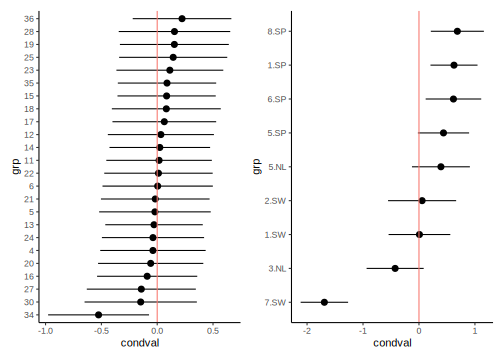
\includegraphics{BIO8940_book_files/figure-latex/unnamed-chunk-64-1.pdf}
\caption{\label{fig:unnamed-chunk-64}Distribution of BLUPs for genotypes and populations}
\end{figure}

As expected from the similarity of the variance estimates, the population-level estimates (the only shared component) do not differ much between the two models. There is a hint of regional differentiation --- the Spanish populations have higher fruit sets than the Swedish and Dutch populations. Genotype 34 again looks a little bit unusual.

\hypertarget{fixed-effects}{%
\subsubsection{Fixed effects}\label{fixed-effects}}

Now we want to do inference on the fixed effects. We use the drop1 func- tion to assess both the AIC difference and the likelihood ratio test between models. (In glmm\_funs.R we define a convenience function dfun to convert the AIC tables returned by drop1 (which we will create momentarily) into ∆AIC tables.) Although the likelihood ratio test (and the AIC) are asymptotic tests, comparing fits between full and reduced models is still more accurate than the Wald (curvature-based) tests shown in the summary tables for glmer fits.

\begin{Shaded}
\begin{Highlighting}[]
\NormalTok{(dd_aic <-}\StringTok{ }\KeywordTok{dfun}\NormalTok{(}\KeywordTok{drop1}\NormalTok{(mp4)))}
\end{Highlighting}
\end{Shaded}

\begin{verbatim}
## Warning in checkConv(attr(opt, "derivs"), opt$par, ctrl = control$checkConv, :
## Model failed to converge with max|grad| = 0.00763683 (tol = 0.002, component 1)
\end{verbatim}

\begin{verbatim}
## Single term deletions
## 
## Model:
## total.fruits ~ nutrient + amd + rack + status + (1 | X) + (1 | 
##     gen) + (1 | popu) + nutrient:amd
##              npar   dAIC
## <none>             0.000
## rack            1 55.081
## status          2  1.611
## nutrient:amd    1  1.443
\end{verbatim}

\begin{Shaded}
\begin{Highlighting}[]
\NormalTok{(dd_lrt <-}\StringTok{ }\KeywordTok{drop1}\NormalTok{(mp4, }\DataTypeTok{test =} \StringTok{"Chisq"}\NormalTok{))}
\end{Highlighting}
\end{Shaded}

\begin{verbatim}
## Warning in checkConv(attr(opt, "derivs"), opt$par, ctrl = control$checkConv, :
## Model failed to converge with max|grad| = 0.00763683 (tol = 0.002, component 1)
\end{verbatim}

\begin{verbatim}
## Single term deletions
## 
## Model:
## total.fruits ~ nutrient + amd + rack + status + (1 | X) + (1 | 
##     gen) + (1 | popu) + nutrient:amd
##              npar    AIC    LRT   Pr(Chi)    
## <none>            5015.4                     
## rack            1 5070.5 57.081 4.182e-14 ***
## status          2 5017.0  5.611   0.06047 .  
## nutrient:amd    1 5016.8  3.443   0.06353 .  
## ---
## Signif. codes:  0 '***' 0.001 '**' 0.01 '*' 0.05 '.' 0.1 ' ' 1
\end{verbatim}

On the basis of these comparisons, there appears to be a very strong effect of rack and weak effects of status and of the interaction term. Dropping the nutrient:amd interaction gives a (slightly) increased AIC (∆AIC = 1.4), so the full model has the best expected predictive capability (by a small margin). On the other hand, the p-value is slightly above 0.05 (p = 0.06). At this point we remove the non-significant interaction term so we can test the main effects. (We don't worry about removing status because it measures an aspect of experimental design that we want to leave in the model whether it is significant or not.) Once we have fitted the reduced model, we can run the LRT via anova.

\begin{Shaded}
\begin{Highlighting}[]
\NormalTok{mp5 <-}\StringTok{ }\KeywordTok{update}\NormalTok{(mp4, . }\OperatorTok{~}\StringTok{ }\NormalTok{. }\OperatorTok{-}\StringTok{ }\NormalTok{amd}\OperatorTok{:}\NormalTok{nutrient)}
\end{Highlighting}
\end{Shaded}

\begin{verbatim}
## Warning in checkConv(attr(opt, "derivs"), opt$par, ctrl = control$checkConv, :
## Model failed to converge with max|grad| = 0.00763683 (tol = 0.002, component 1)
\end{verbatim}

\begin{Shaded}
\begin{Highlighting}[]
\KeywordTok{anova}\NormalTok{(mp5, mp4)}
\end{Highlighting}
\end{Shaded}

\begin{verbatim}
## Data: dat_tf
## Models:
## mp5: total.fruits ~ nutrient + amd + rack + status + (1 | X) + (1 | 
## mp5:     gen) + (1 | popu)
## mp4: total.fruits ~ nutrient + amd + rack + status + (1 | X) + (1 | 
## mp4:     gen) + (1 | popu) + nutrient:amd
##     npar    AIC    BIC  logLik deviance  Chisq Df Pr(>Chisq)  
## mp5    9 5016.8 5056.8 -2499.4   4998.8                       
## mp4   10 5015.4 5059.8 -2497.7   4995.4 3.4427  1    0.06353 .
## ---
## Signif. codes:  0 '***' 0.001 '**' 0.01 '*' 0.05 '.' 0.1 ' ' 1
\end{verbatim}

\textbf{Exercise}
Test now the reduced model.

In the reduced model, we find that both nutrients and clipping have strong effects, whether measured by AIC or LRT. If we wanted to be still more careful about our interpretation, we would try to relax the asymptotic assumption. In classical linear models, we would do this by doing F tests with the appropriate denominator degrees of freedom. In ``modern'' mixed model approaches, we might try to use denominator-degree-of-freedom approximations such as the Kenward-Roger (despite the controversy over these approximations, they are actually available in \texttt{lmerTest}, but they do not apply to GLMMs. We can use a parametric bootstrap comparison between nested models to test fixed effects, as we did above for random effects, with the caveat that is computationally slow.

In addition, we can check the normality of the random effects and find they are reasonable (Fig. 10).

\begin{Shaded}
\begin{Highlighting}[]
\NormalTok{r5 <-}\StringTok{ }\KeywordTok{as.data.frame}\NormalTok{(}\KeywordTok{ranef}\NormalTok{(mp5))}
\KeywordTok{ggplot}\NormalTok{(}\DataTypeTok{data =}\NormalTok{ r5, }\KeywordTok{aes}\NormalTok{(}\DataTypeTok{sample =}\NormalTok{ condval)) }\OperatorTok{+}
\StringTok{  }\KeywordTok{geom_qq}\NormalTok{() }\OperatorTok{+}\StringTok{ }\KeywordTok{geom_qq_line}\NormalTok{() }\OperatorTok{+}
\StringTok{  }\KeywordTok{facet_wrap}\NormalTok{(}\OperatorTok{~}\StringTok{ }\NormalTok{grpvar) }\OperatorTok{+}
\StringTok{  }\KeywordTok{theme_classic}\NormalTok{()}
\end{Highlighting}
\end{Shaded}

\begin{figure}
\centering
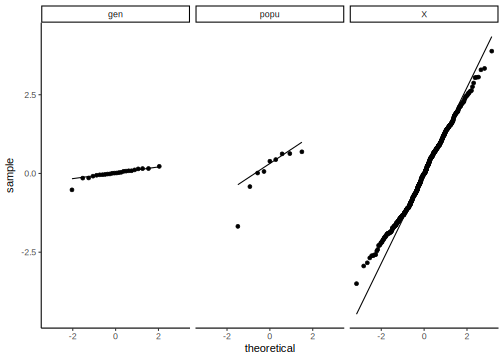
\includegraphics{BIO8940_book_files/figure-latex/unnamed-chunk-67-1.pdf}
\caption{\label{fig:unnamed-chunk-67}Q-Q plot of BLUPs from model mp5}
\end{figure}

\hypertarget{conclusions}{%
\subsection{Conclusions}\label{conclusions}}

Our final model includes fixed effects of nutrients and clipping, as well as the nuisance variables rack and status; observation-level random effects to ac- count for overdispersion; and variation in overall fruit set at the population and genotype levels. However, we don't (apparently) have quite enough in- formation to estimate the variation in clipping and nutrient effects, or their interaction, at the genotype or population levels. There is a strong overall positive effect of nutrients and a slightly weaker negative effect of clipping. The interaction between clipping and nutrients is only weakly supported (i.e.~the p-value is not very small), but it is positive and about the same magnitude as the clipping effect, which is consistent with the statement that ``nutrients cancel out the effect of herbivory''.

\begin{rmdcode}
\textbf{Exercise}

\begin{itemize}
\tightlist
\item
  Re-do the analysis with region as a fixed effect.
\item
  Re-do the analysis with a one-way layout as suggested above
\end{itemize}
\end{rmdcode}

\hypertarget{happy-generalized-mixed-modelling}{%
\subsection{Happy generalized mixed-modelling}\label{happy-generalized-mixed-modelling}}

\begin{figure}

{\centering 
\includegraphics[width=0.5\linewidth]{images/Thorn} 

}

\caption{A GLMM character}\label{fig:unnamed-chunk-69}
\end{figure}

\backmatter

\hypertarget{part-appendix}{%
\part{Appendix}\label{part-appendix}}

\hypertarget{r-1}{%
\chapter*{R}\label{r-1}}
\addcontentsline{toc}{chapter}{R}

Need to write something about R

We also use various methods for manipulating and visualising data frames using the 📦 \texttt{tidyverse} \citep{R-tidyverse} (including \texttt{tidyr}, \texttt{dplyr}, \texttt{ggplot2} etc).
You can get more details on their use can be found at in the Book \texttt{R\ for\ Data\ Science} \citep{wickhamDataScienceImport2016} which is freely available as a \href{http://r4ds.had.co.nz/}{bookdown website here}.

\hypertarget{to-do-list}{%
\chapter*{To do list}\label{to-do-list}}
\addcontentsline{toc}{chapter}{To do list}

\begin{itemize}
\tightlist
\item
  clean code
\item
  add more info about allEffects and plotting prediction of models
\item
  convert all plots to ggplot
\item
  convert data handling to tidyverse
\item
  finish chapters
\end{itemize}

  \bibliography{book.bib,packages.bib}

\printindex

\end{document}
